\documentclass[UTF8]{ctexart}
\usepackage{ctex}
\usepackage{graphicx}
\usepackage{color}
\usepackage{xcolor}
\usepackage{listings}
\usepackage{float}
\usepackage{amsmath}
\usepackage{tikz}
\usepackage{pgfplots}
\usepackage{fancyhdr}
\usepackage{mdframed}
\usepackage{caption}
\usepackage{ booktabs}
\usepackage{makecell}
\usepackage{amsthm}
\usepackage{hyperref }
\usepackage{ pgffor }
\usepackage{caption}
\usepackage{subcaption}
\usepackage{fancyhdr}
\usepackage{graphicx}
\usepackage{geometry} % 页面边距设置
\geometry{left=2.5cm, right=2.5cm, top=2.5cm, bottom=2.5cm}


%================================================================================================================%
\begin{document}

% 插入图片,调整宽度为页面宽度
\begin{center}
    
\includegraphics[width=\textwidth]{o} % 替换为您的图片文件名
\end{center}

% 定义标题
\begin{center}
    \huge\textbf{第三周实验报告}
\end{center}

% 定义作者
\begin{center}
    \huge\textbf{於佳杰}
\end{center}
% 以下内容将从下一页开始
\newpage
\title{第三周实验报告}
\author{於佳杰}
\date{2024 年 9 月 10 日}
\maketitle
\pagenumbering{arabic}
\tableofcontents
\newpage


\pagenumbering{arabic}

\pagestyle{fancy}
\fancyhf{}
\renewcommand{\headrulewidth}{1pt}
\renewcommand{\footrulewidth}{1pt}
\fancyhead[L]{
\includegraphics[width=1.5cm]{okkl}} % 确保图片路径正确
\fancyhead[C]{\rightmark}
\fancyfoot[C]{\thepage}
\fancyhead[R]{\thepage}







% 1实验目的================================================================================================%

\section{实验目的}
{\color{red}掌握命令行环境,Python入门基础,Python视觉应用。}

\section{实例展示}
{\color{red}进行命令行环境,Python入门基础,Python视觉应用实例展示。}
%1.2LaTex=========================================================================%
  \subsection{命令行环境}
  {\color{blue}命令行环境命令展示}



%1.1LaTex=========================================================================%
%1.8LaTex=========================================================================%
\subsubsection{后台执行作业}

\begin{enumerate}
  \item 使用一些命令来获取 Job 的 PID,然后杀死它们
  \begin{itemize}
  \item 命令展示
  \begin{verbatim}

sleep 10000 &


pid=$!


echo "Process ID: $pid"
pgrep -f "sleep 10000"

pkill -f "sleep 10000"


pgrep -f "sleep 10000"  

  \end{verbatim}
\item 效果展示
 \begin{figure}[H]
    \centering
    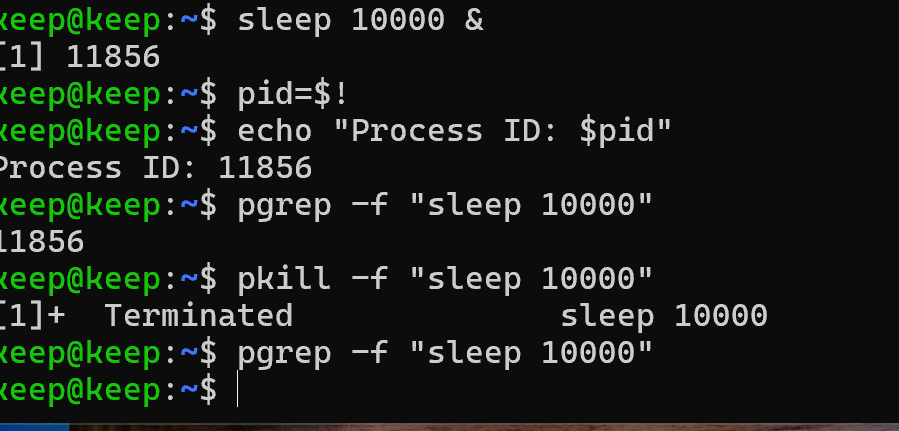
\includegraphics[width=\textwidth]{1} % 替换为您的图片文件名
    \caption{列表效果展示}
  \end{figure}
  \end{itemize}
\end{enumerate}

%1.9LaTex=========================================================================%
%1.8LaTex=========================================================================%
\subsubsection{获取最常用的 10 个命令}

\begin{enumerate}
  \item 获取最常用的 10 个命令
  \begin{itemize}
  \item 命令展示
  \begin{verbatim}
history | awk '{$1="";print substr($0,2)}' | sort | uniq -c | sort -n | tail -n 10


  \end{verbatim}
\item 效果展示
 \begin{figure}[H]
    \centering
    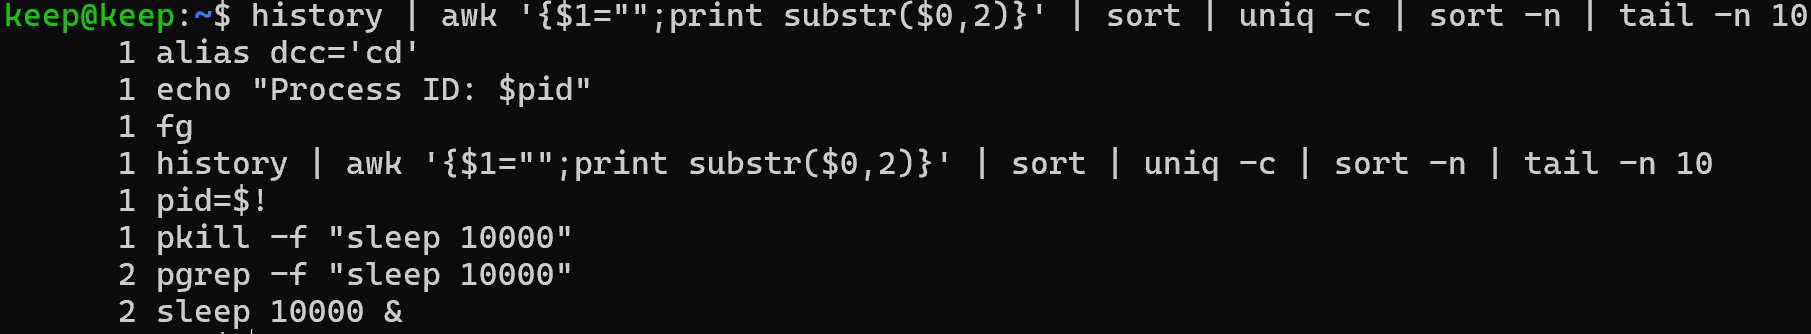
\includegraphics[width=\textwidth]{2} % 替换为您的图片文件名
    \caption{列表效果展示}
  \end{figure}
  \end{itemize}
\end{enumerate}

%1.9LaTex=========================================================================%
%1.8LaTex=========================================================================%
\subsubsection{VM 中安装 mosh 并建立连接}

\begin{enumerate}
  \item VM 中安装 mosh 并建立连接,然后断开服务器/VM 的网络适配器。mosh 能从中适当恢复吗
  \begin{itemize}
  \item 命令展示
  \begin{verbatim}
ssh keep@192.168.43.128

sudo apt update
sudo apt install mosh
mosh keep@192.168.43.128
断网
mosh keep@192.168.43.128
ssh -N -f -L 8080:localhost:80 keep@192.168.43.128
能恢复
  \end{verbatim}
\item 效果展示
 \begin{figure}[H]
    \centering
    \begin{subfigure}[b]{0.48\textwidth}
        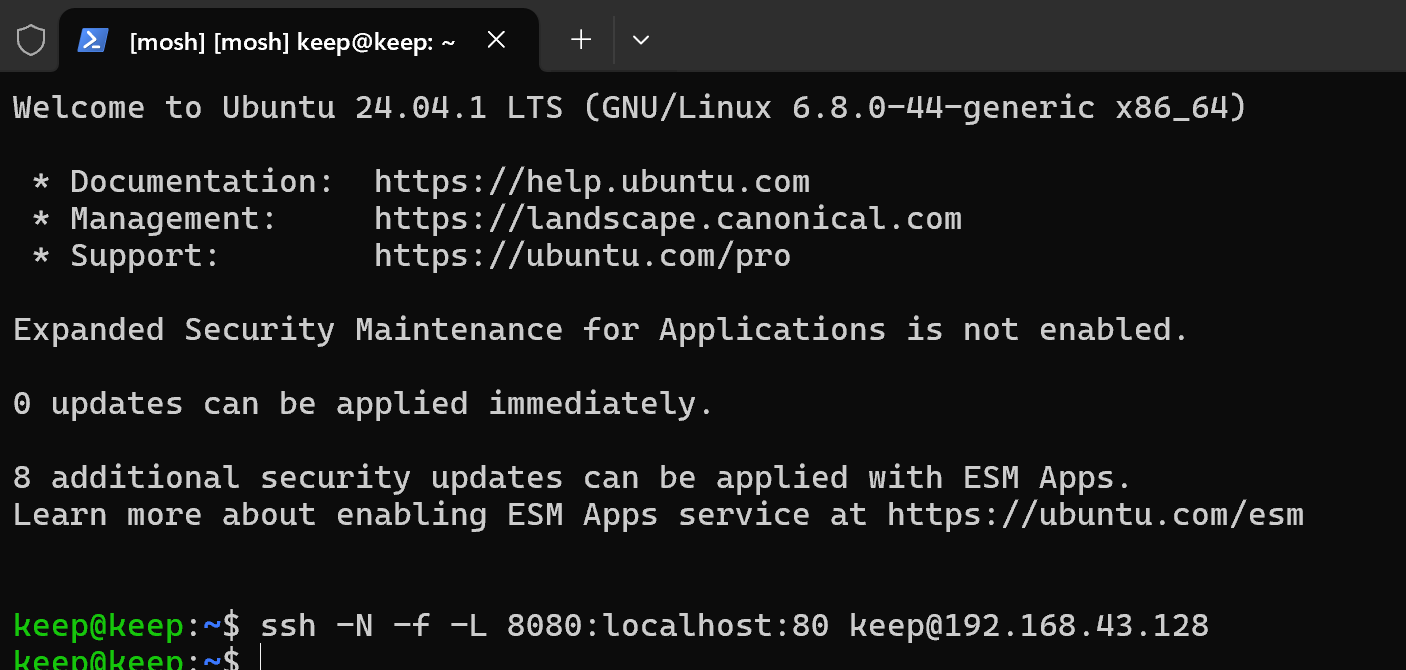
\includegraphics[width=\textwidth]{121} % 替换为您的第一张图片文件名
        \caption{效果}
        \label{fig:left}
    \end{subfigure}
    \hfill
    \begin{subfigure}[b]{0.48\textwidth}
        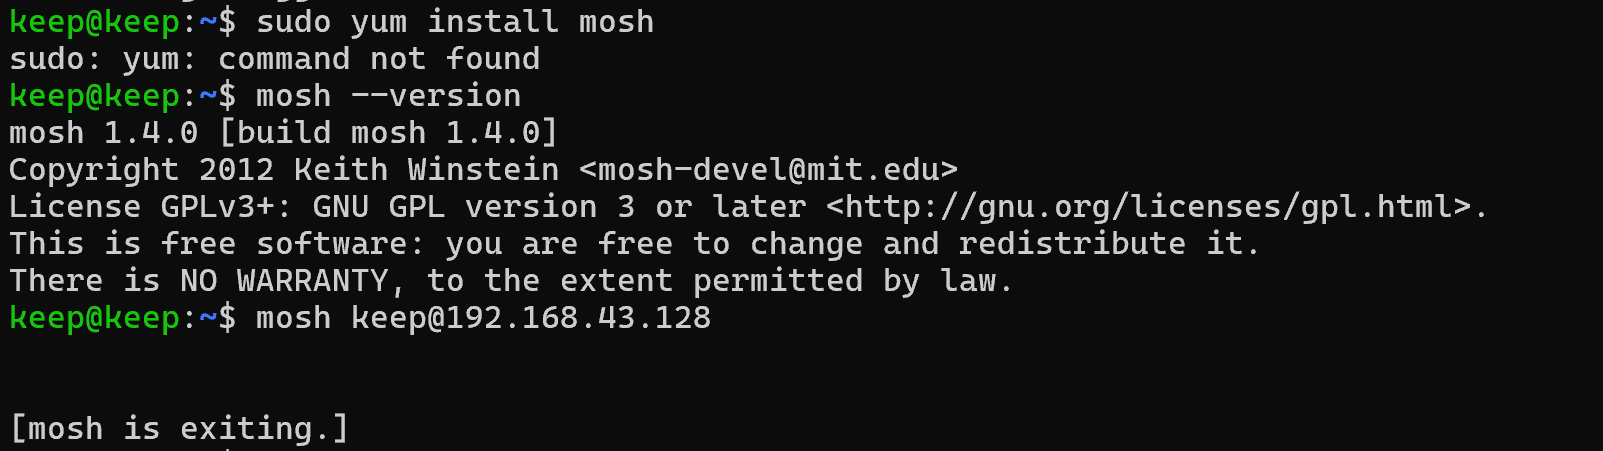
\includegraphics[width=\textwidth]{122} % 替换为您的第二张图片文件名
        \caption{效果}
        \label{fig:right}
    \end{subfigure}
    \caption{效果展示}
    \label{fig:side_by_side}
\end{figure}
  \end{itemize}
\end{enumerate}

%1.9LaTex=========================================================================%


%1.9LaTex=========================================================================%
\subsubsection{结束进程}

\begin{enumerate}
  \item 结束进程并使用 Python 程序展示了捕获信号 SIGINT 并忽略它的基本操作
  \begin{itemize}
  \item 命令展示
  \begin{verbatim}
sleep 20
 Ctrl-C
#!/usr/bin/env python
import signal, time

def handler(signum, time):
    print("\nI got a SIGINT, but I am not stopping")

signal.signal(signal.SIGINT, handler)
i = 0
while True:
    time.sleep(.1)
    print("\r{}".format(i), end="")
    i += 1
 Ctrl-C
Ctrl-\
  \end{verbatim}
\item 效果展示
  \begin{figure}[H]
    \centering
    \begin{subfigure}[b]{0.48\textwidth}
        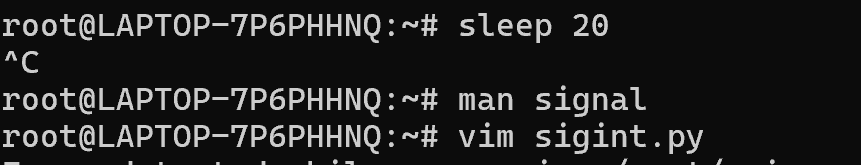
\includegraphics[width=\textwidth]{11} % 替换为您的第一张图片文件名
        \caption{效果}
        \label{fig:left}
    \end{subfigure}
    \hfill
    \begin{subfigure}[b]{0.48\textwidth}
        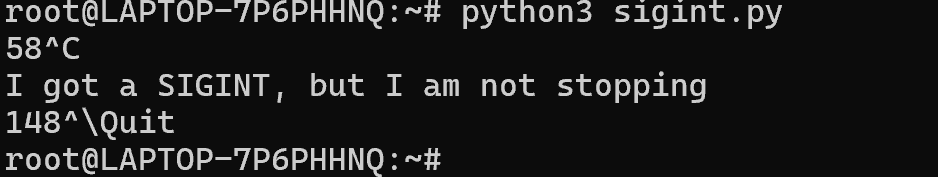
\includegraphics[width=\textwidth]{1111} % 替换为您的第二张图片文件名
        \caption{效果}
        \label{fig:right}
    \end{subfigure}
    \caption{效果展示}
    \label{fig:side_by_side}
\end{figure}
  \end{itemize}
\end{enumerate}


%1.2LaTex=========================================================================%
\subsubsection{暂停和后台执行进程}

\begin{enumerate}
  \item 信号可以让进程做其他的事情,而不仅仅是终止它们。
  \begin{itemize}
  \item 命令展示
  \begin{verbatim}
 sleep 1000
^Z
nohup sleep 2000 &
 bg \%1
 jobs
 kill -STOP \%1
 kill -HUP \%1
 kill -HUP \%2
 kill -KILL \%2
jobs
  \end{verbatim}
\item 效果展示
  \begin{figure}[H]
    \centering
    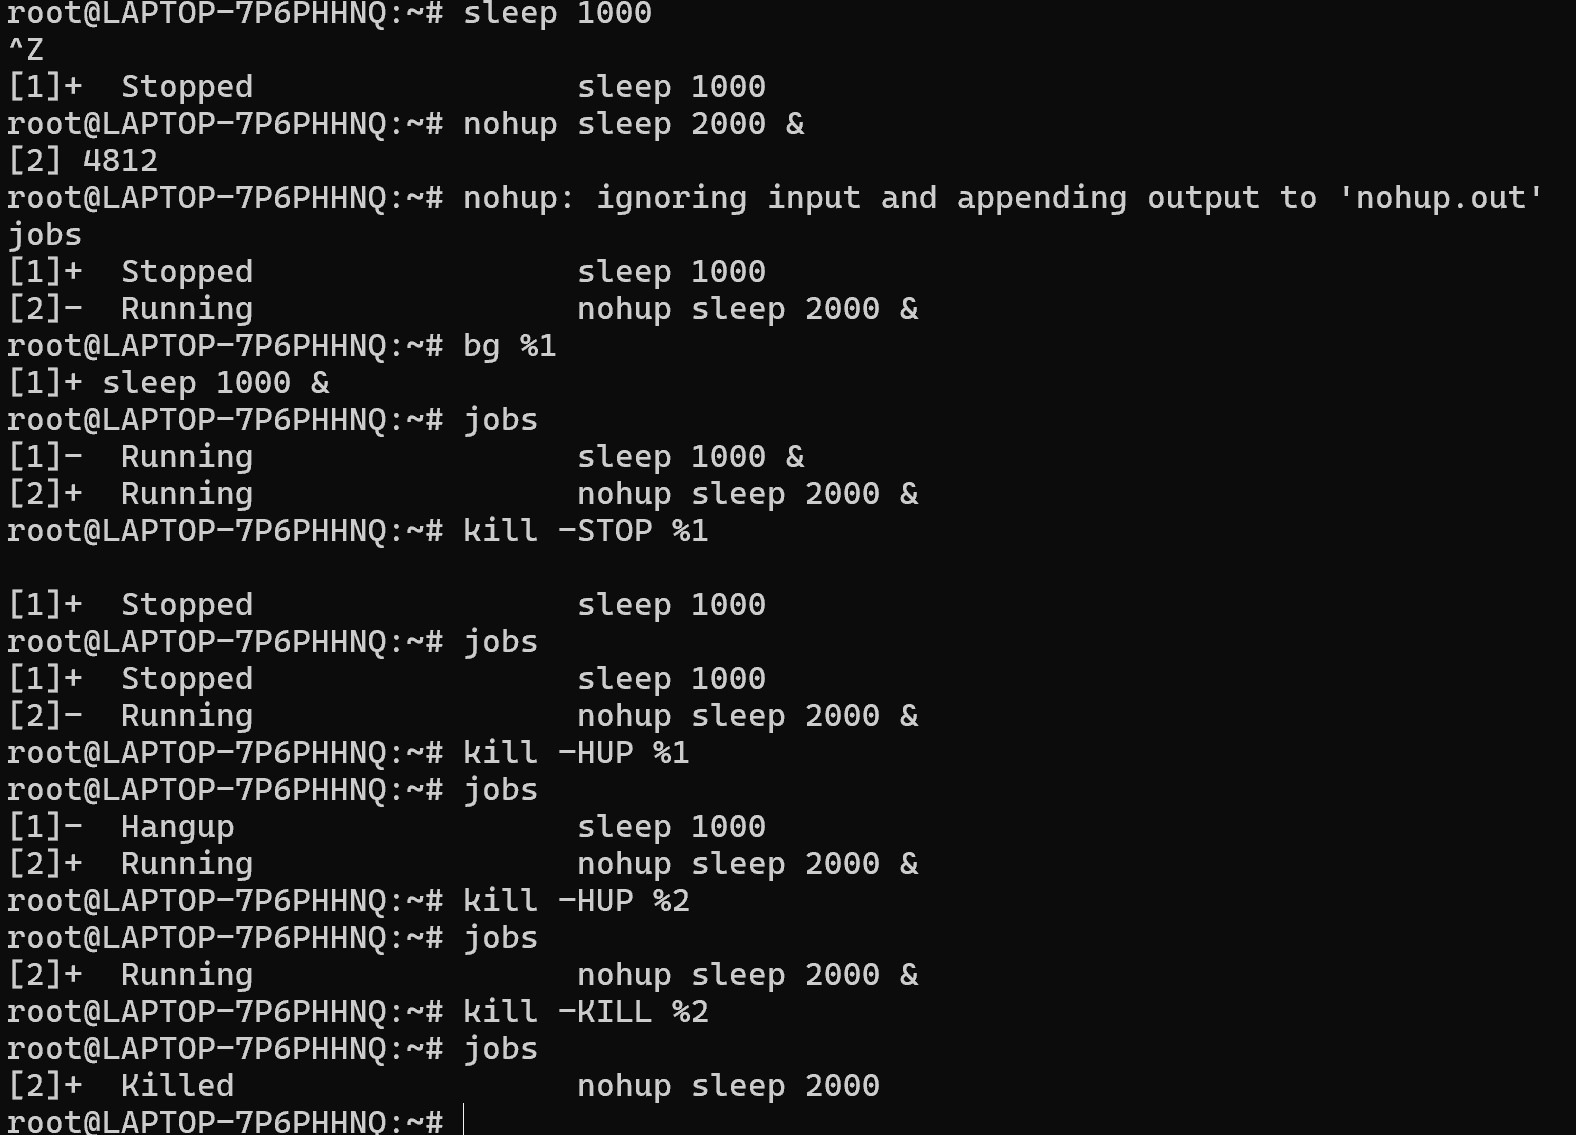
\includegraphics[width=\textwidth]{12} % 替换为您的图片文件名
    \caption{列表效果展示}
  \end{figure}
  \end{itemize}
\end{enumerate}

%1.3LaTex=========================================================================%
\subsubsection{终端多路复用}

\begin{enumerate}
  \item 使用终端多路复用器
  \begin{itemize}
  \item 命令展示
  \begin{verbatim}
tmux 开始一个新的会话
tmux new -s NAME 以指定名称开始一个新的会话
tmux ls 列出当前所有会话
 <C-b> d 将当前会话分离
tmux a 重新连接最后一个会话。
<C-b> " 水平分割
<C-b> \% 垂直分割
<C-b> z 切换当前面板的缩放
  \end{verbatim}\item 效果展示
\begin{figure}[H]
    \centering
    \begin{subfigure}[b]{0.48\textwidth}
        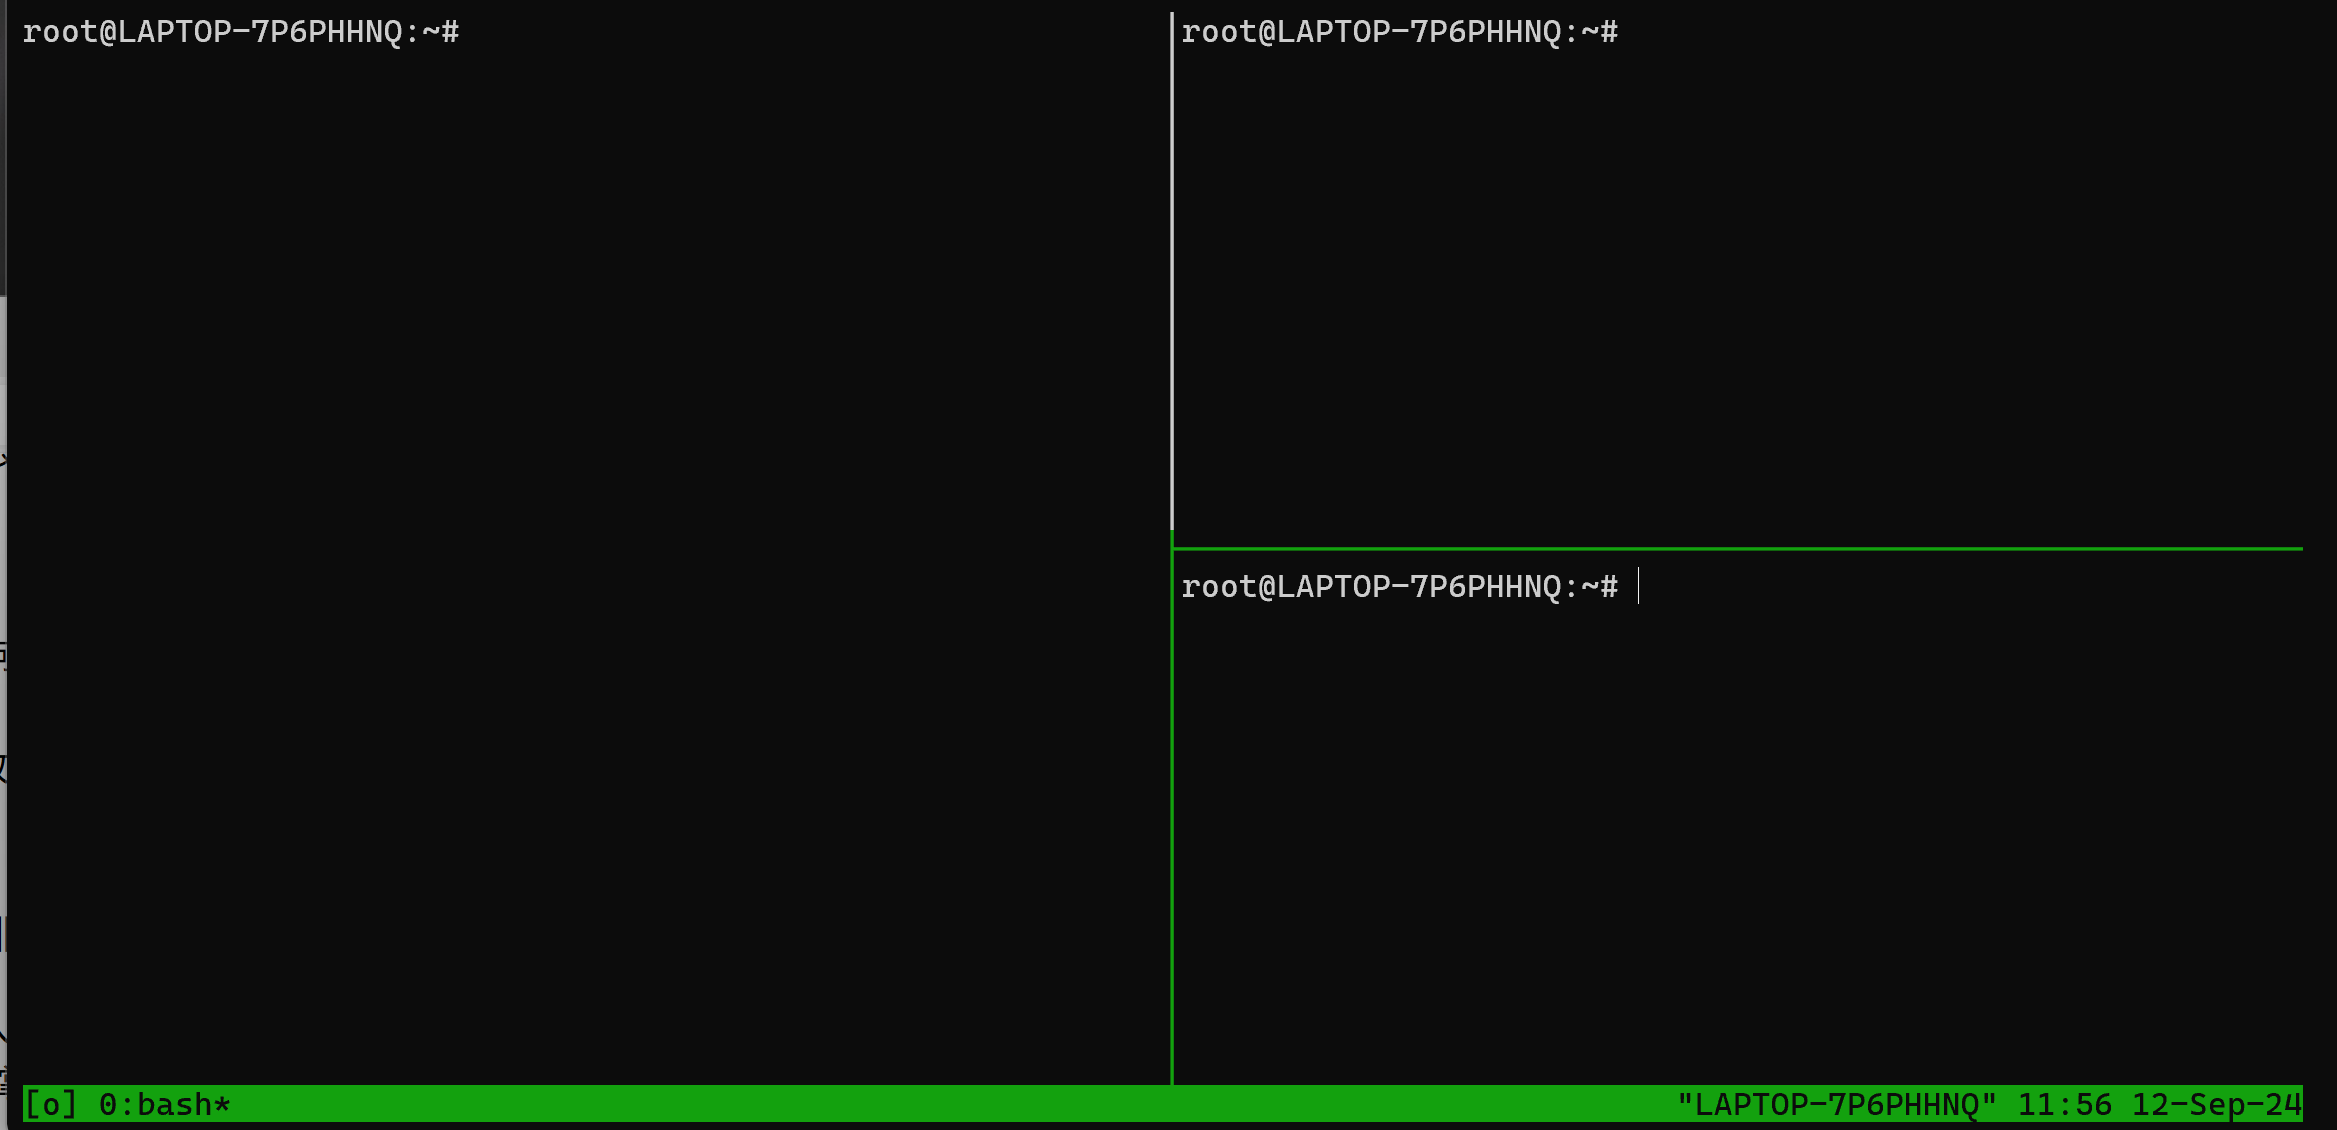
\includegraphics[width=\textwidth]{13} % 替换为您的第一张图片文件名
        \caption{效果}
        \label{fig:left}
    \end{subfigure}
    \hfill
    \begin{subfigure}[b]{0.48\textwidth}
        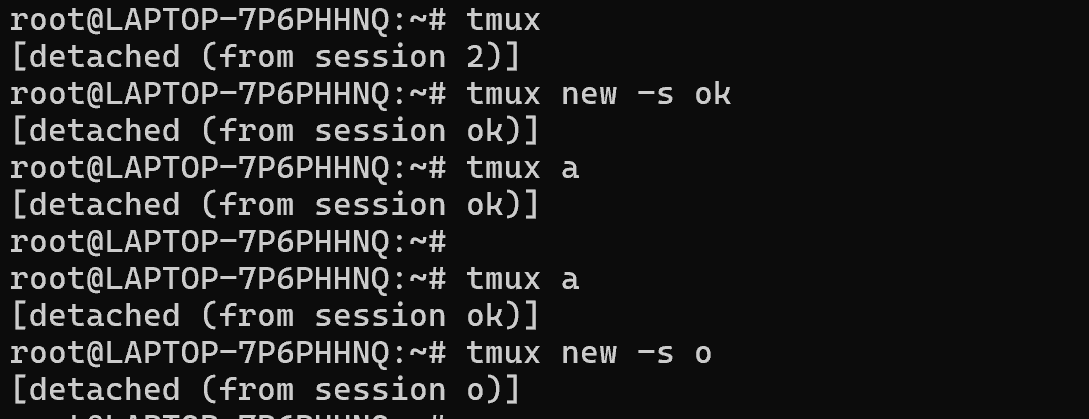
\includegraphics[width=\textwidth]{14} % 替换为您的第二张图片文件名
        \caption{效果}
        \label{fig:right}
    \end{subfigure}
    \caption{效果展示}
    \label{fig:side_by_side}
\end{figure}

  \end{itemize}
\end{enumerate}
%1.4LaTex=========================================================================%
\subsubsection{别名}

\begin{enumerate}
  \item 相当于缩写,能够少输入很多
  \begin{itemize}
  \item 命令展示
  \begin{verbatim}
alias ll="ls -lh"
alias gs="git status"
alias gc="git commit"
alias v="vim"
alias sl=ls
alias mv="mv -i"           \# -i prompts before overwrite
alias mkdir="mkdir -p"     \# -p make parent dirs as needed
alias df="df -h"   
alias la="ls -A"
alias lla="la -l"
禁用别名
unalias la
忽略某个别名
\ls
获取别名的定义
alias ll
  \end{verbatim}
\item 效果展示
  \begin{figure}[H]
    \centering
    \begin{subfigure}[b]{0.48\textwidth}
        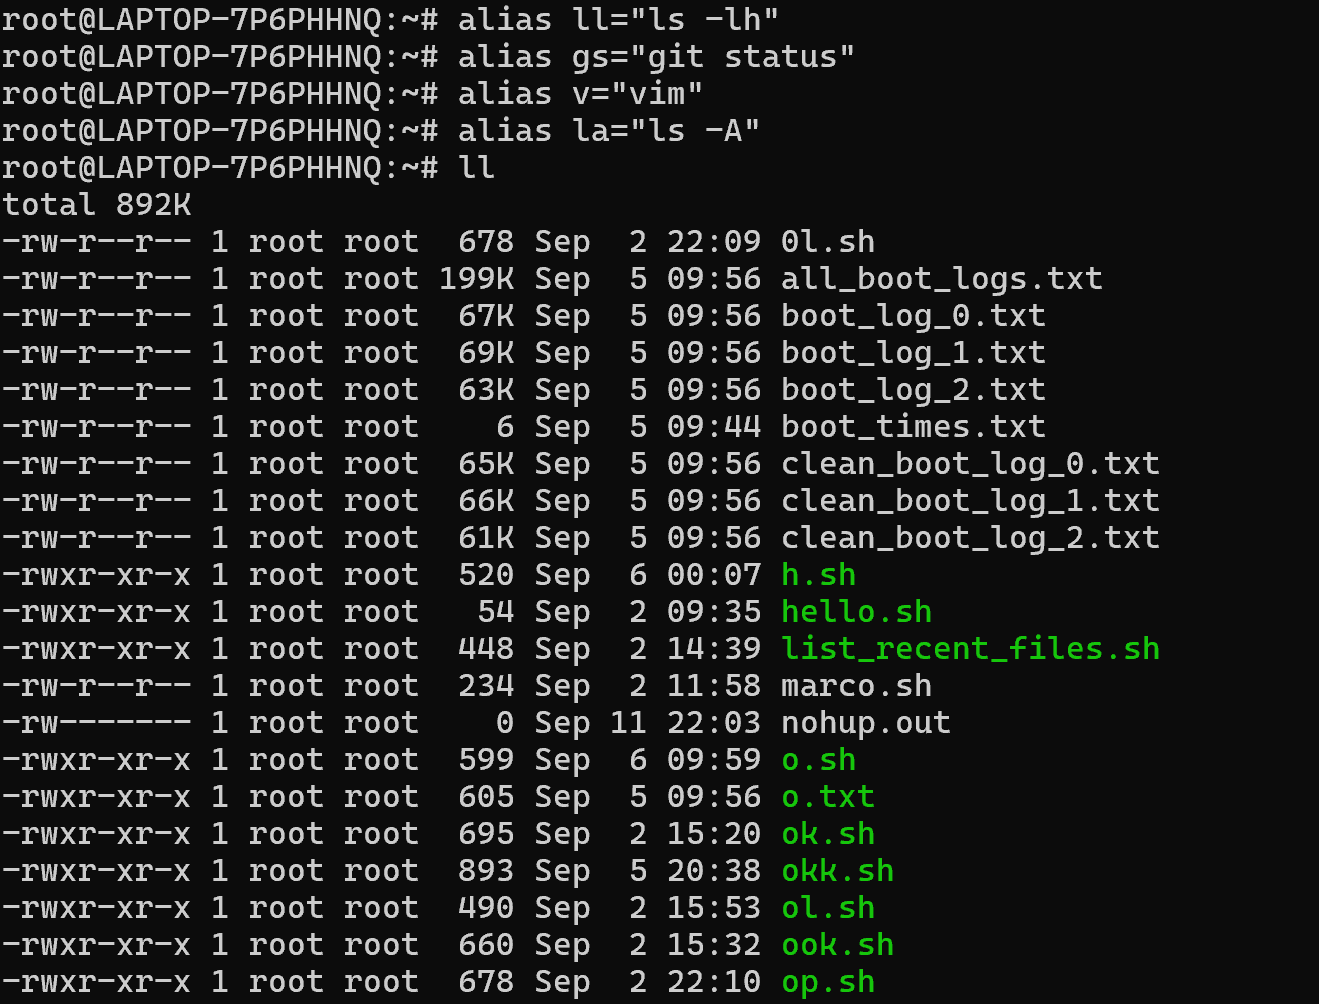
\includegraphics[width=\textwidth]{141} % 替换为您的第一张图片文件名
        \caption{效果}
        \label{fig:left}
    \end{subfigure}
    \hfill
    \begin{subfigure}[b]{0.48\textwidth}
        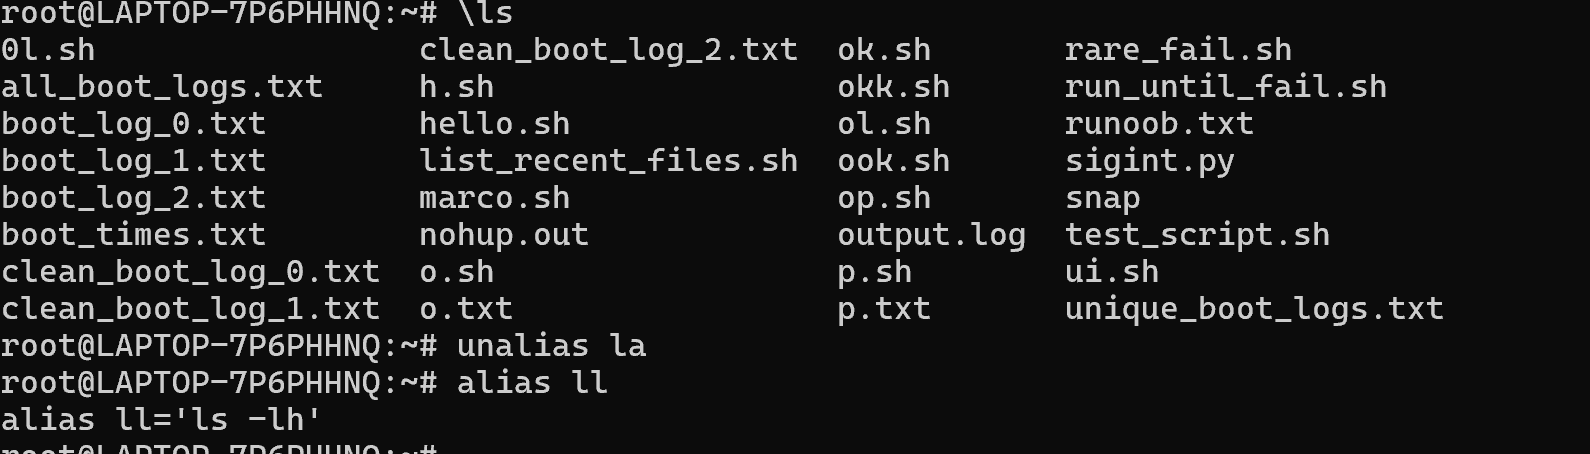
\includegraphics[width=\textwidth]{142} % 替换为您的第二张图片文件名
        \caption{效果}
        \label{fig:right}
    \end{subfigure}
    \caption{效果展示}
    \label{fig:side_by_side}
\end{figure}
  \end{itemize}
\end{enumerate}

%1.5LaTex=========================================================================%
\subsubsection{使用SSH执行命令}

\begin{enumerate}
  \item 使用SSH执行命令
  \begin{itemize}
  \item 命令展示
  \begin{verbatim}
ssh keep@192.168.43.128 
ssh keep@192.168.43.128 'ls'
ssh keep@192.168.43.128 'ls' | grep PATTERN
ls | ssh keep@192.168.43.128 'grep PATTERN'

  \end{verbatim}
\item 效果展示
  \begin{figure}[H]
    \centering
    \begin{subfigure}[b]{0.48\textwidth}
        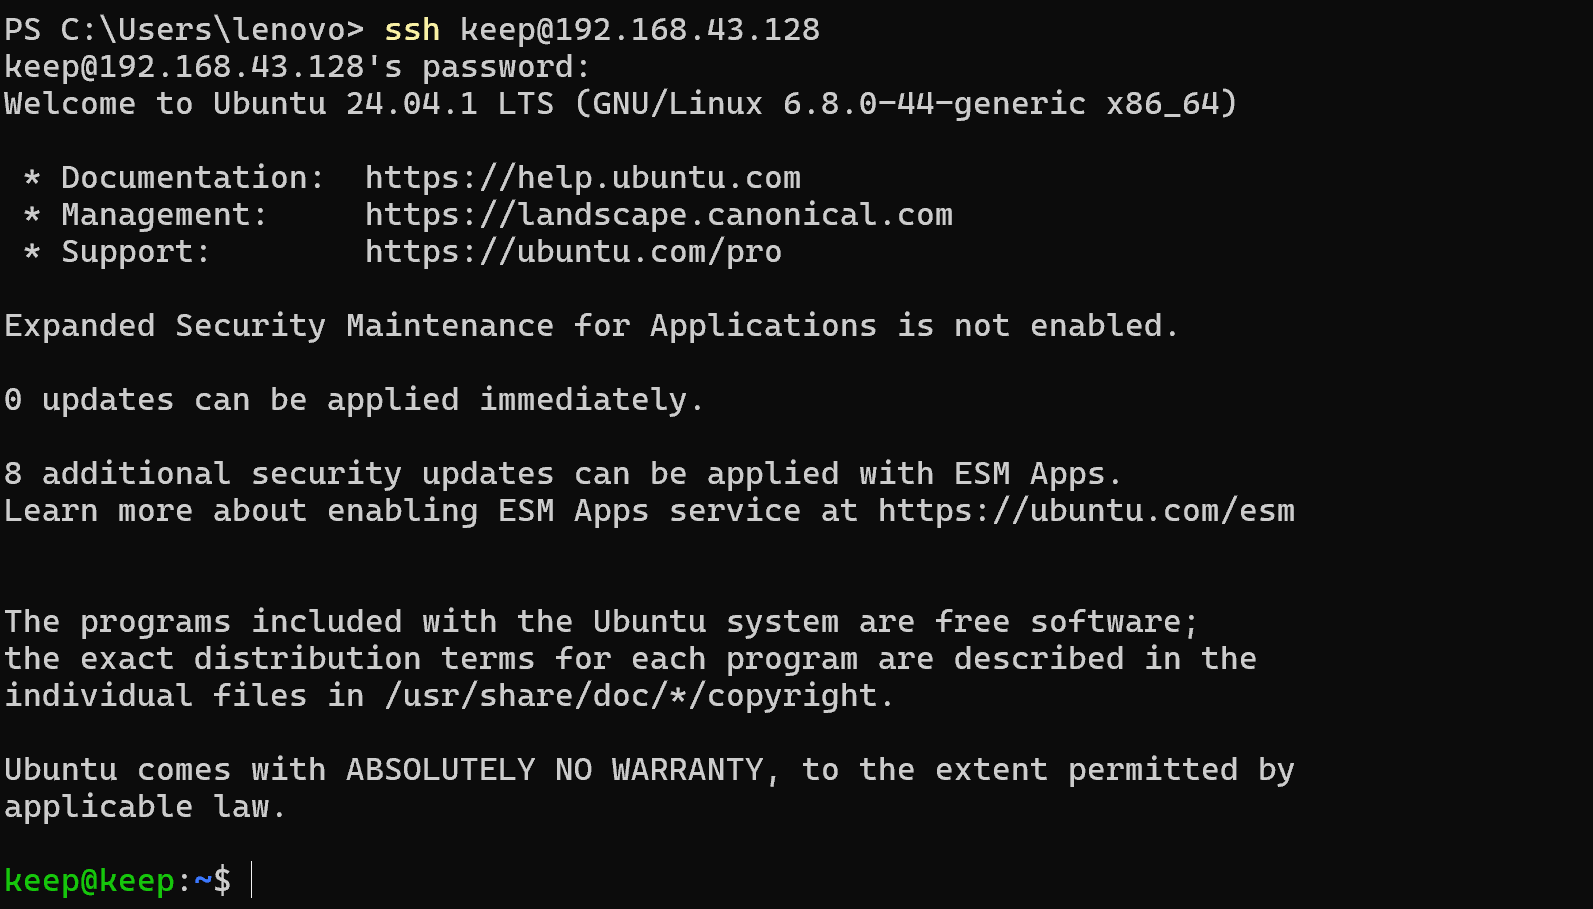
\includegraphics[width=\textwidth]{115} % 替换为您的第一张图片文件名
        \caption{效果}
        \label{fig:left}
    \end{subfigure}
    \hfill
    \begin{subfigure}[b]{0.48\textwidth}
        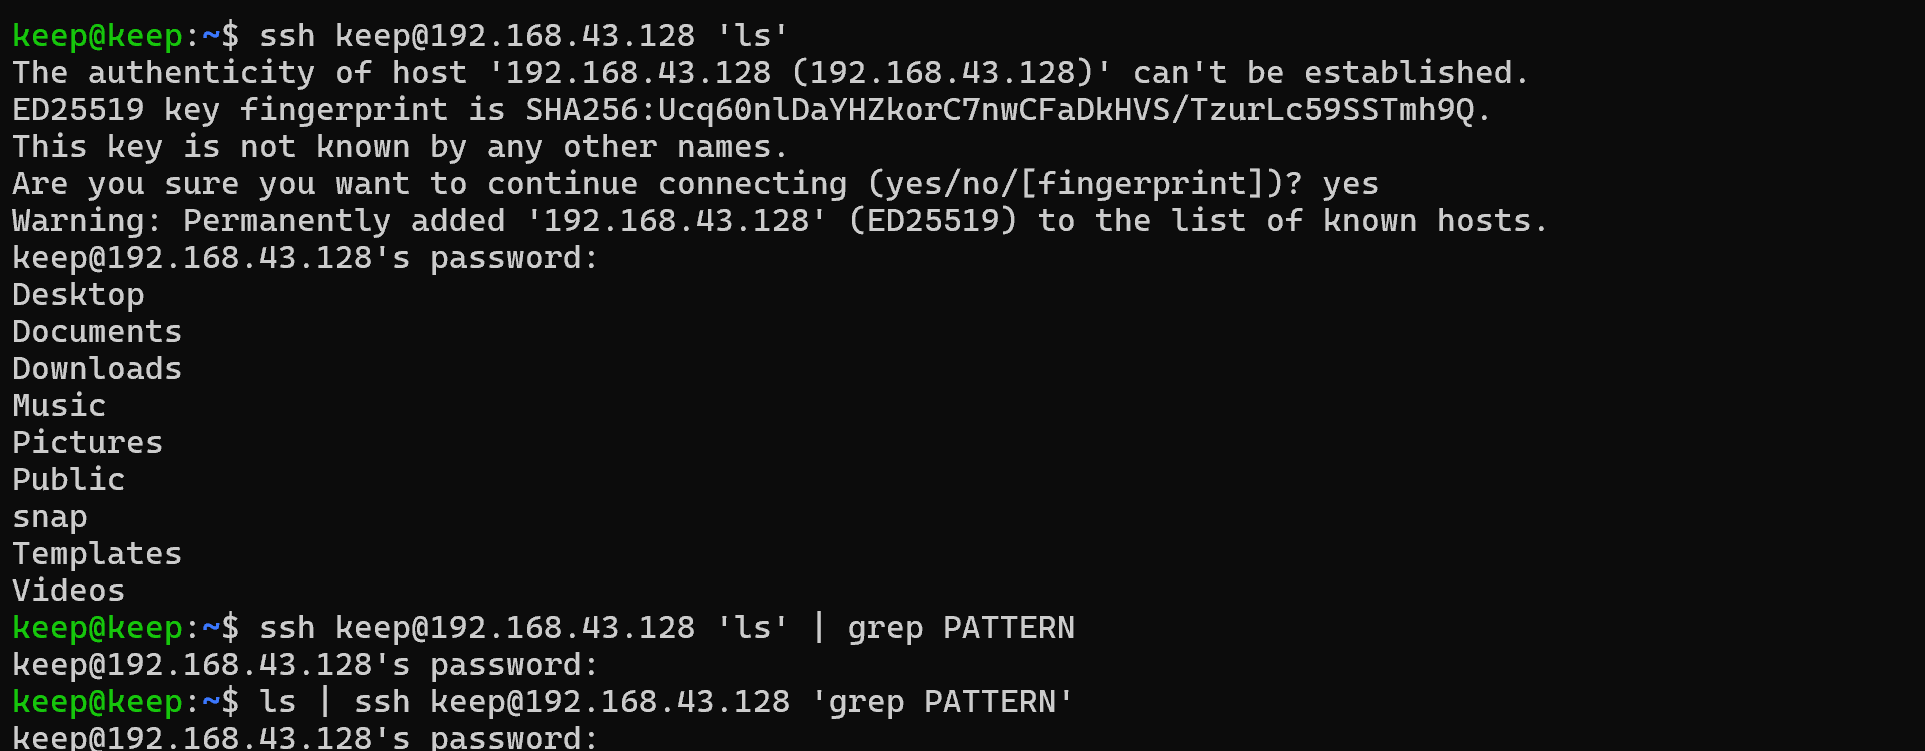
\includegraphics[width=\textwidth]{116} % 替换为您的第二张图片文件名
        \caption{效果}
        \label{fig:right}
    \end{subfigure}
    \caption{效果展示}
    \label{fig:side_by_side}
\end{figure}
  \end{itemize}
\end{enumerate}

%1.6LaTex=========================================================================%
\subsubsection{SSH 密钥}

\begin{enumerate}
  \item 利用公钥加密向服务器证明客户端拥有秘密私钥,而无需泄露密钥,实现免密登录
  \begin{itemize}
  \item 命令展示
  \begin{verbatim}
ssh-keygen -o -a 100 -t ed25519 -f ~/.ssh/id_ed25519
ssh-keygen -y -f ~/.ssh/id_ed25519
cat ~/.ssh/id_ed25519.pub | ssh keep@192.168.43.128 'cat >> ~/.ssh/authorized_keys'
ssh-copy-id -i ~/.ssh/id_ed25519.pub keep@192.168.43.128

  \end{verbatim}
\item 效果展示
  \begin{figure}[H]
    \centering
    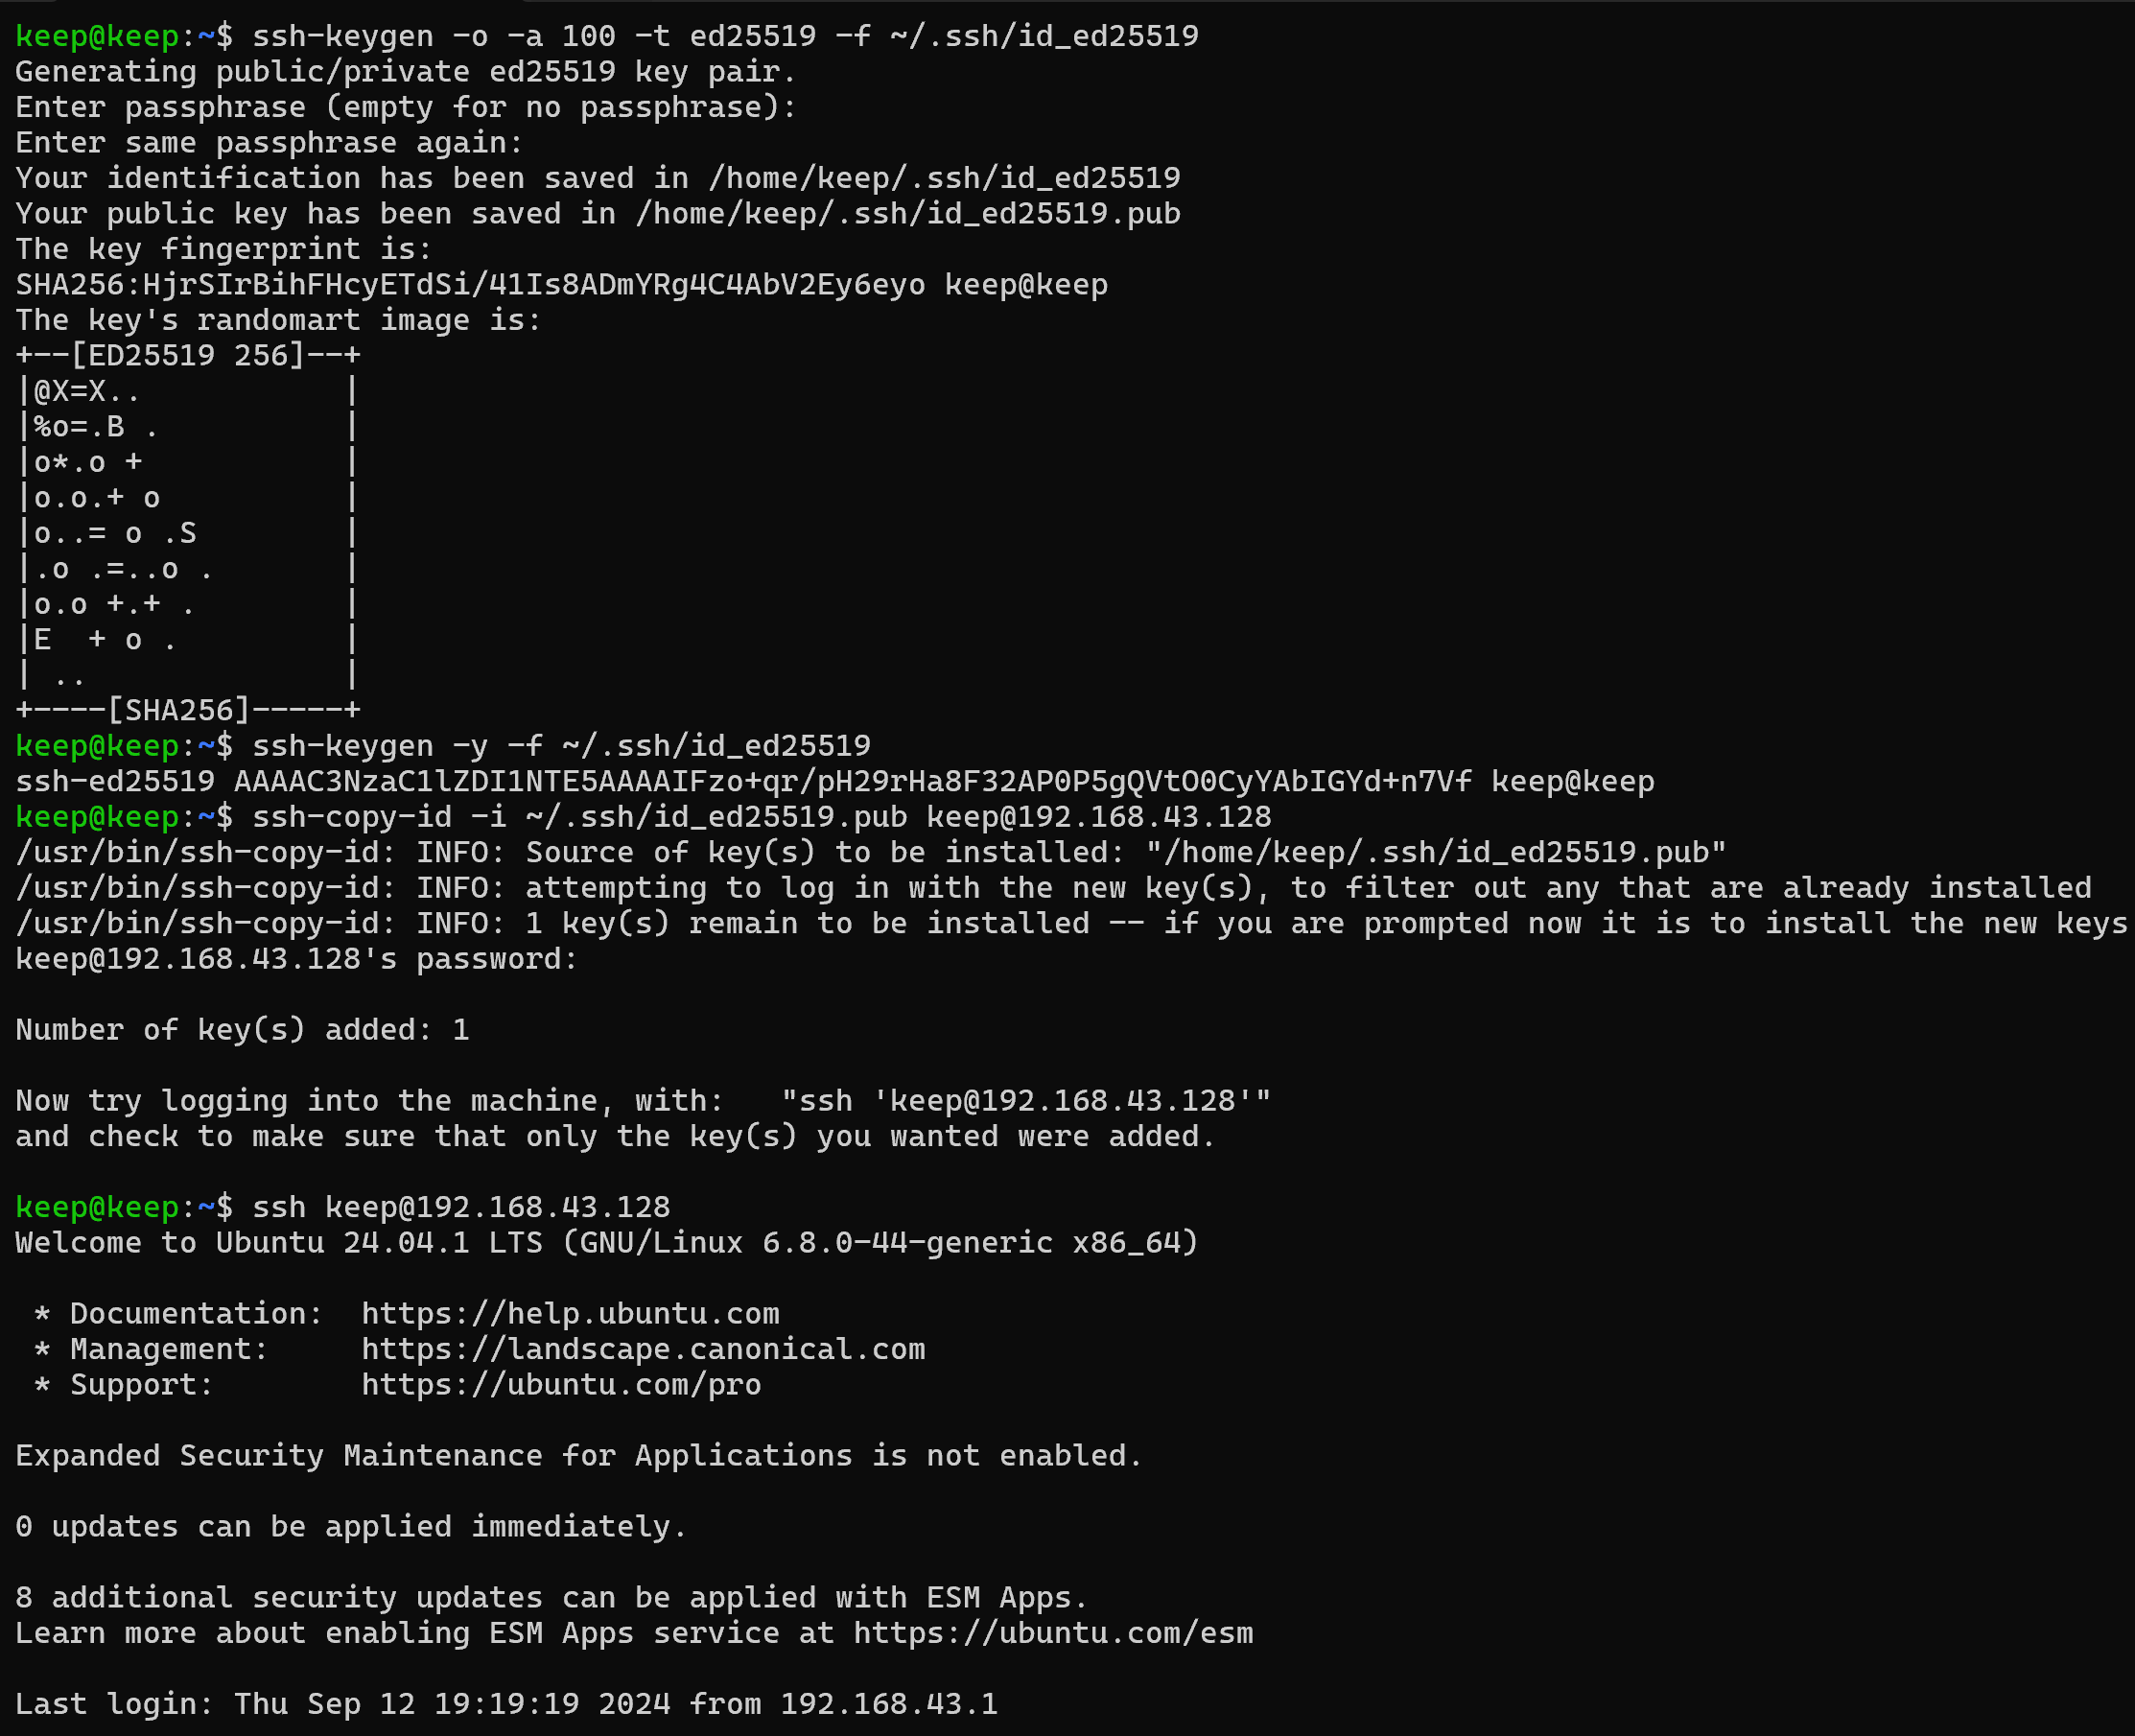
\includegraphics[width=\textwidth]{1116} % 替换为您的图片文件名
    \caption{列表效果展示}
  \end{figure}
  \end{itemize}
\end{enumerate}

%1.7LaTex=========================================================================%
\subsubsection{通过 SSH 复制文件}

\begin{enumerate}
  \item 通过 SSH 复制文件
  \begin{itemize}
  \item 命令展示
  \begin{verbatim}
echo "Hello, this is a test file." > localfile
cat localfile | ssh keep@192.168.43.128 'tee serverfile'
scp localfile keep@192.168.43.128:~/serverfile_copy
ssh keep@192.168.43.128 'cat ~/serverfile_copy'

  \end{verbatim}
\item 效果展示
  \begin{figure}[H]
    \centering
    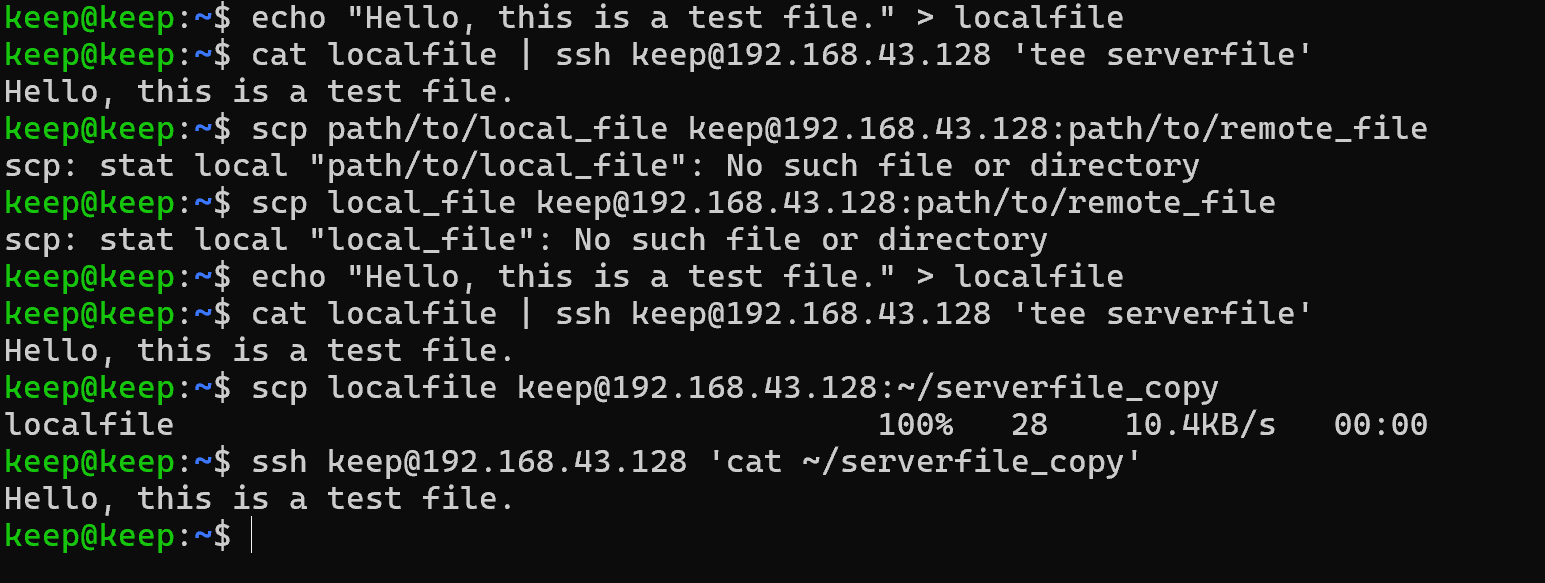
\includegraphics[width=\textwidth]{117} % 替换为您的图片文件名
    \caption{列表效果展示}
  \end{figure}
  \end{itemize}
\end{enumerate}

%1.8LaTex=========================================================================%
\subsubsection{端口转发}

\begin{enumerate}
  \item 进行本地端口转发和远程端口转发
  \begin{itemize}
  \item 命令展示
  \begin{verbatim}
ssh -L 9999:localhost:8888 keep@192.168.43.128
ssh -R 8888:localhost:9999 keep@192.168.43.128

  \end{verbatim}
\item 效果展示
 \begin{figure}[H]
    \centering
    \begin{subfigure}[b]{0.48\textwidth}
        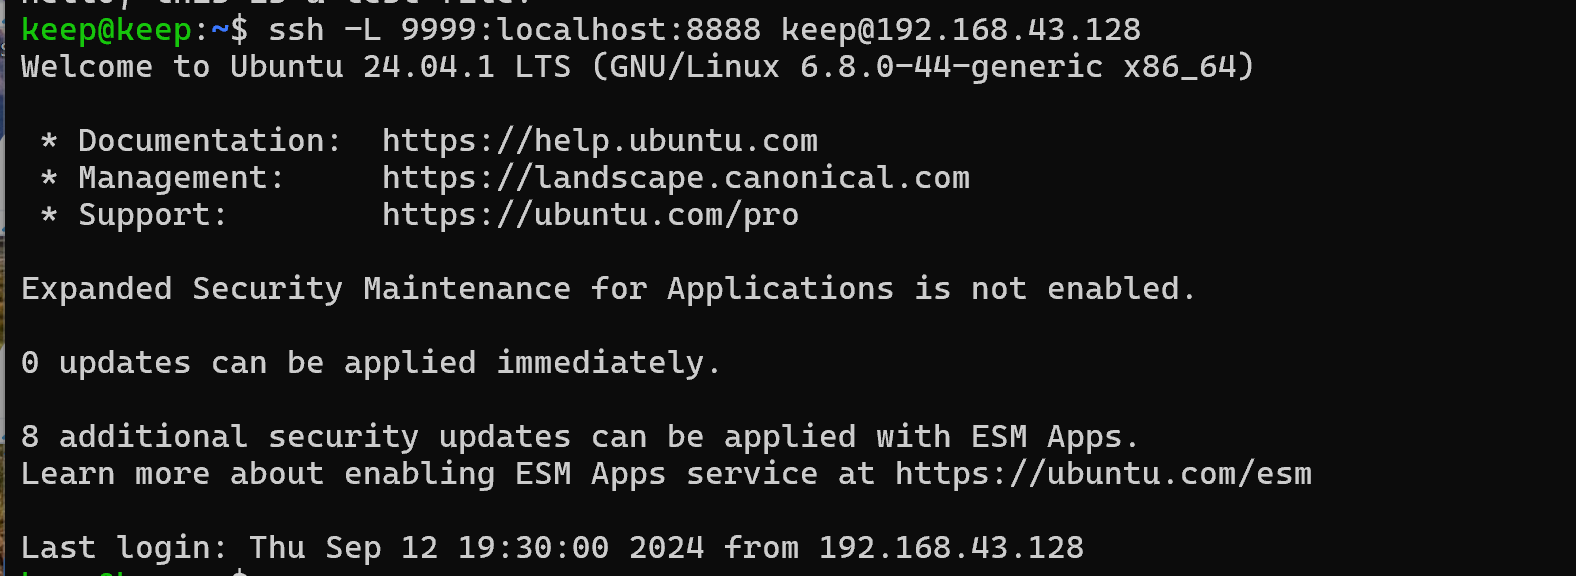
\includegraphics[width=\textwidth]{181} % 替换为您的第一张图片文件名
        \caption{效果}
        \label{fig:left}
    \end{subfigure}
    \hfill
    \begin{subfigure}[b]{0.48\textwidth}
        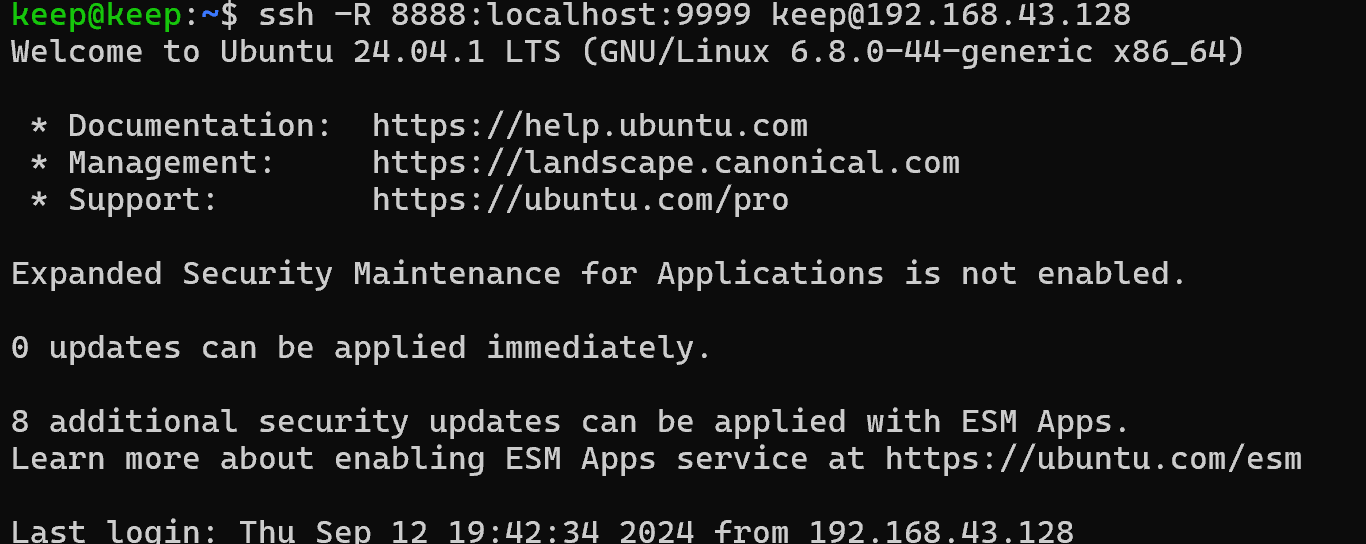
\includegraphics[width=\textwidth]{182} % 替换为您的第二张图片文件名
        \caption{效果}
        \label{fig:right}
    \end{subfigure}
    \caption{效果展示}
    \label{fig:side_by_side}
\end{figure}
  \end{itemize}
\end{enumerate}

%1.9LaTex=========================================================================%
\subsubsection{压缩与解压}

\begin{enumerate}
  \item 使用 tar 压缩与解压
  \begin{itemize}
  \item 命令展示
  \begin{verbatim}
# 创建示例目录
mkdir example_directory

# 进入目录
cd example_directory

# 创建一些示例文件
echo "This is file 1." > file1.txt
echo "This is file 2." > file2.txt
echo "This is file 3." > file3.txt

# 查看创建的文件
ls
# 返回上级目录
cd ..

# 创建压缩档案
tar -czvf archive.tar.gz example_directory
tar -tzvf archive.tar.gz
tar -xzvf archive.tar.gz
ls example_directory

  \end{verbatim}
\item 效果展示
  \begin{figure}[H]
    \centering
    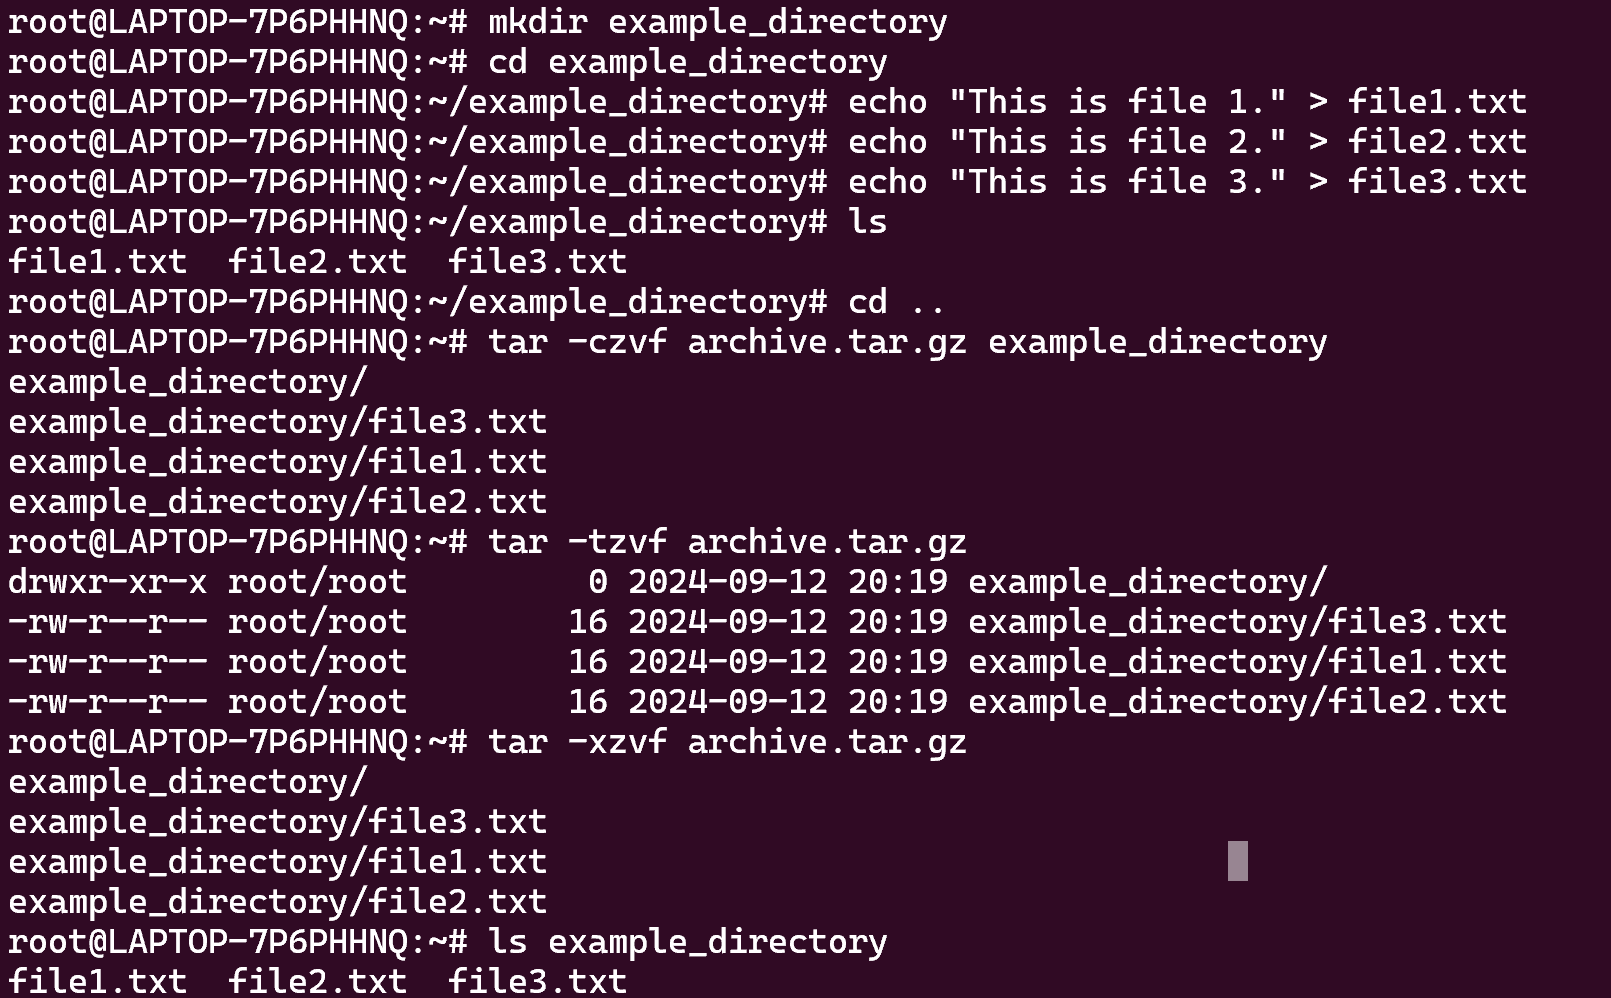
\includegraphics[width=\textwidth]{19} % 替换为您的图片文件名
    \caption{列表效果展示}
  \end{figure}
  \end{itemize}
\end{enumerate}

%1.10LaTex=========================================================================%
\subsubsection{ 批量重命名文件}

\begin{enumerate}
  \item 批量重命名文件,添加前缀或后缀。
  \begin{itemize}
  \item 命令展示
  \begin{verbatim}
touch test1.jpg test2.jpg
for file in *.jpg; do mv "$file" "newprefix_$file"; done
ls


  \end{verbatim}
\item 效果展示
  \begin{figure}[H]
    \centering
    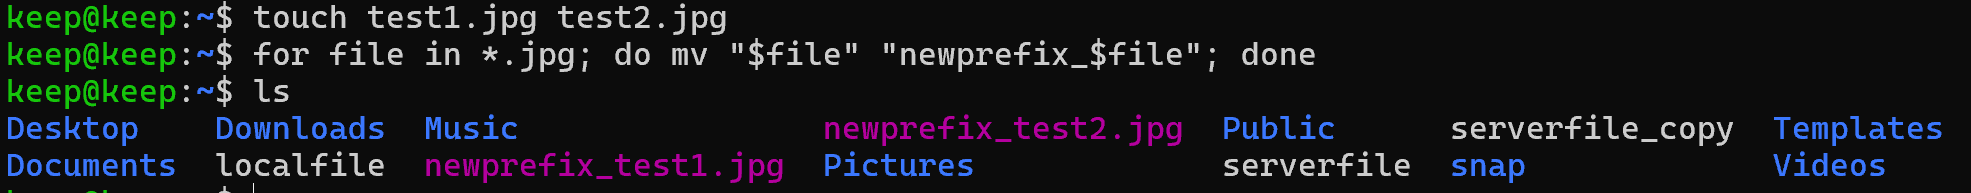
\includegraphics[width=\textwidth]{10} % 替换为您的图片文件名
    \caption{列表效果展示}
  \end{figure}
  \end{itemize}
\end{enumerate}

%1.11LaTex=========================================================================%
\subsubsection{网络工具}

\begin{enumerate}
  \item 使用 ping 检查网络
  \begin{itemize}
  \item 命令展示
  \begin{verbatim}
ping google.com
  \end{verbatim}
\item 效果展示
  \begin{figure}[H]
    \centering
    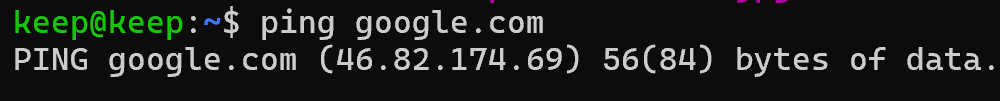
\includegraphics[width=\textwidth]{101} % 替换为您的图片文件名
    \caption{列表效果展示}
  \end{figure}
  \end{itemize}
\end{enumerate}


































































%1.2LaTex=========================================================================%
  \subsection{Python入门基础}
  {\color{blue}Python入门基础展示}











%2.1LaTex=========================================================================%
\subsubsection{列表}

\begin{enumerate}
  \item 定义列表,打印列表并进行一些简单操作
  \begin{itemize}
  \item 命令展示
  \begin{verbatim}
list = [1, 2, 3, 'frist', 9.0]
ok = [99, 'I am ']
ok.extend(list)
print(list)
print(list[0])
print(list[1:3])
print(list[2:])
print(ok * 2)
print(list + ok)
print(ok)
print(ok.index('frist'))
print(ok.count('frist'))
print(ok.pop(2))
print(ok)
ok.reverse()
print(ok)

    
  \end{verbatim}

  \item 效果展示
  \begin{figure}[H]
    \centering
    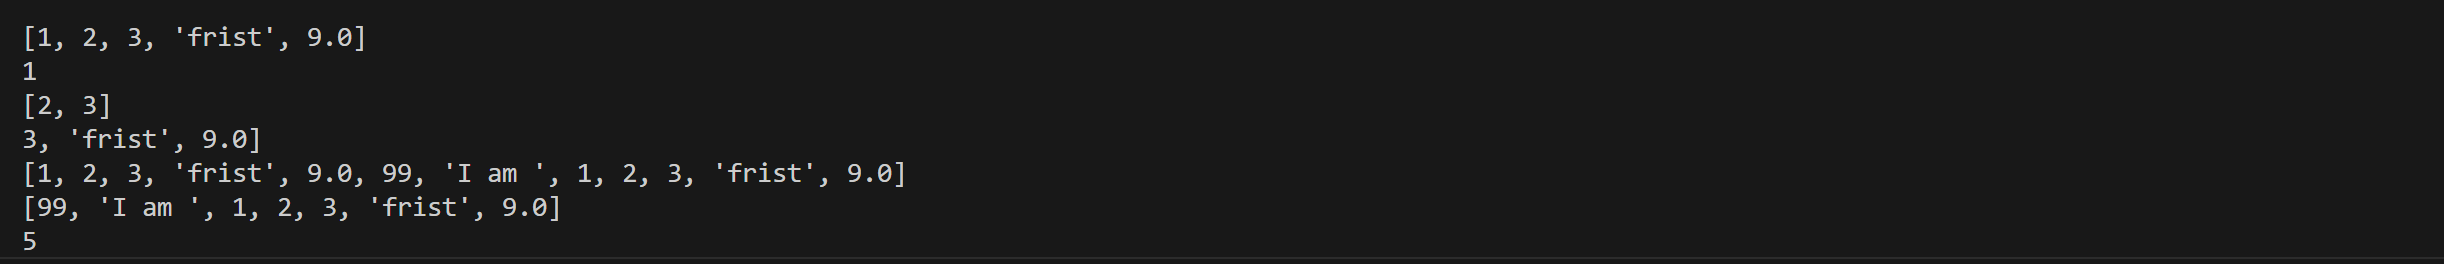
\includegraphics[width=\textwidth]{21} % 确保文件名正确
    \caption{效果展示}
  
  \end{figure}
  \begin{figure}[H]
    \centering
    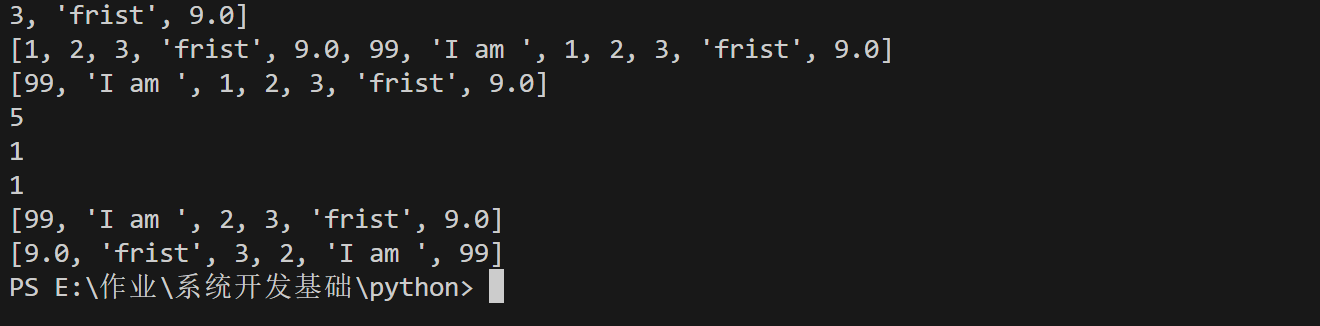
\includegraphics[width=\textwidth]{211} % 确保文件名正确
    \caption{效果展示}
  
  \end{figure}
\end{itemize}
\end{enumerate}
















%2.2LaTex=========================================================================%
\subsubsection{元组}

\begin{enumerate}
  \item 定义元组,打印元组并进行一些简单操作
  \begin{itemize}
  \item 命令展示
  \begin{verbatim}

tup1 = (12, 34.56)
tup2 = ('abc', 'xyz')

tup3 = tup1 + tup2
print(tup3)
print(tup1 * 2)
print(len(tup3))
print(tup3.count('abc'))
print(tup3.index('xyz'))
print(tup3.index(34.56))

del tup1

print(tup3[1:4])

    
  \end{verbatim}

  \item 效果展示
  \begin{figure}[H]
    \centering
    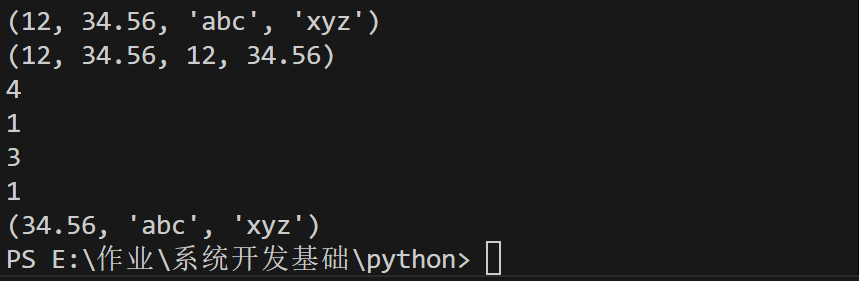
\includegraphics[width=\textwidth]{22} % 确保文件名正确
    \caption{效果展示}
  
  \end{figure}
\end{itemize}
\end{enumerate}




















%2.3LaTex=========================================================================%
\subsubsection{集合}

\begin{enumerate}
  \item 定义集合,打印集合并进行一些简单操作
  \begin{itemize}
  \item 命令展示
  \begin{verbatim}
  set1 = {'apple', 'banana', 'cherry'}
set1.add('date')
set1.remove('banana')
has_apple = 'apple' in set1

set2 = {'cherry', 'elderberry', 'fig'}
union_set = set1.union(set2)
intersection_set = set1.intersection(set2)
difference_set = set1.difference(set2)
symmetric_difference_set = set1.symmetric_difference(set2)

print(set1)
print(has_apple)
print(union_set)
print(intersection_set)
print(difference_set)
print(symmetric_difference_set)


    
  \end{verbatim}

  \item 效果展示
  \begin{figure}[H]
    \centering
    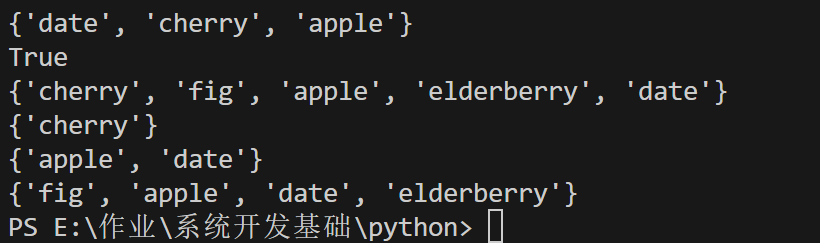
\includegraphics[width=\textwidth]{23} % 确保文件名正确
    \caption{效果展示}
  
  \end{figure}
\end{itemize}
\end{enumerate}
























%2.4LaTex=========================================================================%
\subsubsection{字典}

\begin{enumerate}
  \item 定义集合,打印集合并进行一些简单操作
  \begin{itemize}
  \item 命令展示
  \begin{verbatim}
 

dict1 = {'name': 'Alice', 'age': 30, 'city': 'New York'}


dict1['job'] = 'Engineer'


dict1['age'] = 31


del dict1['city']


keys = dict1.keys()

values = dict1.values()


items = dict1.items()


has_name = 'name' in dict1

city = dict1.get('city', 'Unknown')

print(dict1)           
print(keys)             
print(values)           
print(items)            
print(has_name)       
print(city)             


    
  \end{verbatim}

  \item 效果展示
  \begin{figure}[H]
    \centering
    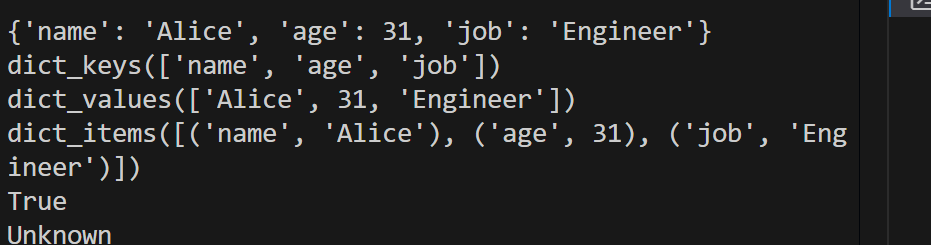
\includegraphics[width=\textwidth]{24} % 确保文件名正确
    \caption{效果展示}
  
  \end{figure}
\end{itemize}
\end{enumerate}

















%2.5LaTex=========================================================================%
\subsubsection{条件控制}

\begin{enumerate}
  \item 条件控制语句展示
  \begin{itemize}
  \item 命令展示
  \begin{verbatim}
  num = int(input("输入一个数字:"))

if num % 2 == 0 and num % 3 == 0:
    print("你输入的数字可以整除 2 和 3")
elif num % 2 == 0:
    print("你输入的数字可以整除 2,但不能整除 3")
elif num % 3 == 0:
    print("你输入的数字可以整除 3,但不能整除 2")
else:
    print("你输入的数字不能整除 2 和 3")


    
  \end{verbatim}

  \item 效果展示
  \begin{figure}[H]
    \centering
    
\includegraphics[width=\textwidth]{25} % 确保文件名正确
    \caption{效果展示}
  
  \end{figure}
\end{itemize}
\end{enumerate}





















%2.6LaTex=========================================================================%
\subsubsection{循环语句}

\begin{enumerate}
  \item 循环语句展示
  \begin{itemize}
  \item 命令展示
  \begin{verbatim}
 \# 第一个实例
for letter in 'okk':
    if letter == 'o':
        continue
    print('当前字母 :', letter)

\# 第二个实例
var = 5
while var > 0:
    var -= 1
    if var == 5:
        continue
    print('当前变量值 :', var)



    
  \end{verbatim}

  \item 效果展示
  \begin{figure}[H]
    \centering
    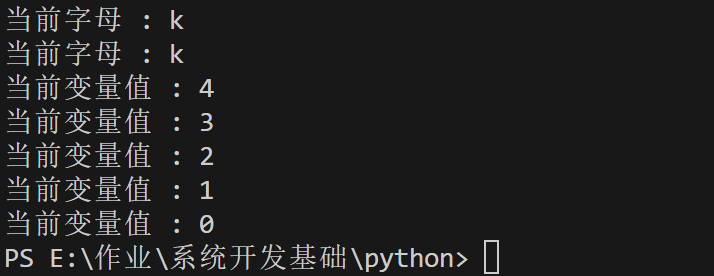
\includegraphics[width=\textwidth]{26} % 确保文件名正确
    \caption{效果展示}
  
  \end{figure}
\end{itemize}
\end{enumerate}






















%2.7LaTex=========================================================================%
\subsubsection{多重赋值 }

\begin{enumerate}
  \item 多重赋值 
  \begin{itemize}
  \item 命令展示
  \begin{verbatim}
 a, b, c = 1, 2, 3
print(a, b, c)

    
  \end{verbatim}

  \item 效果展示
  \begin{figure}[H]
    \centering
    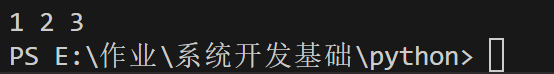
\includegraphics[width=\textwidth]{27} % 确保文件名正确
    \caption{效果展示}
  
  \end{figure}
\end{itemize}
\end{enumerate}




















%2.8LaTex=========================================================================%
\subsubsection{递归函数}

\begin{enumerate}
  \item 简单递归函数展示
  \begin{itemize}
  \item 命令展示
  \begin{verbatim}
 def factorial(n):
    if n == 0:
        return 1
    else:
        return n * factorial(n-1)

print(factorial(5))

    
  \end{verbatim}

  \item 效果展示
  \begin{figure}[H]
    \centering
    
\includegraphics[width=\textwidth]{28} % 确保文件名正确
    \caption{效果展示}
  
  \end{figure}
\end{itemize}
\end{enumerate}






















%2.9LaTex=========================================================================%
\subsubsection{链式比较 }

\begin{enumerate}
  \item 简单链式比较展示
  \begin{itemize}
  \item 命令展示
  \begin{verbatim}
  x = 5
print(1 < x < 10) 

    
  \end{verbatim}

  \item 效果展示
  \begin{figure}[H]
    \centering
    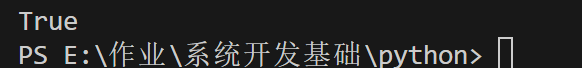
\includegraphics[width=\textwidth]{29} % 确保文件名正确
    \caption{效果展示}
  
  \end{figure}
\end{itemize}
\end{enumerate}





















%2.10LaTex=========================================================================%
\subsubsection{计数器}

\begin{enumerate}
  \item 统计元素出现次数
  \begin{itemize}
  \item 命令展示
  \begin{verbatim}
 from collections import Counter
my_list = ['a', 'b', 'c', 'a', 'b', 'a']
counter = Counter(my_list)
print(counter)
    
  \end{verbatim}

  \item 效果展示
  \begin{figure}[H]
    \centering
    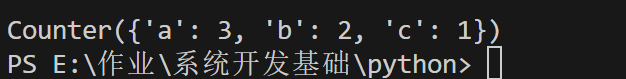
\includegraphics[width=\textwidth]{210} % 确保文件名正确
    \caption{效果展示}
  
  \end{figure}
\end{itemize}
\end{enumerate}

















%2.11LaTex=========================================================================%
\subsubsection{正则表达式}

\begin{enumerate}
  \item 使用正则表达式在字符串中搜索数字
  \begin{itemize}
  \item 命令展示
  \begin{verbatim}
import re

pattern = r'\d+'
string = "The year is 2024."

search_result = re.search(pattern, string)

if search_result:
    print("Found number:", search_result.group())  # 输出 "Found number: 2024"
else:
    print("No number found")


    
  \end{verbatim}

  \item 效果展示
  \begin{figure}[H]
    \centering
    
\includegraphics[width=\textwidth]{2111} % 确保文件名正确
    \caption{效果展示}
  
  \end{figure}
\end{itemize}
\end{enumerate}





%2.12LaTex=========================================================================%
\subsubsection{列表推导式}

\begin{enumerate}
  \item 使用列表推导式生成一个包含 0 到 9 的平方数的列表。
  \begin{itemize}
  \item 命令展示
  \begin{verbatim}
  squares = [x**2 for x in range(10)]
print(squares)

    
  \end{verbatim}

  \item 效果展示
  \begin{figure}[H]
    \centering
    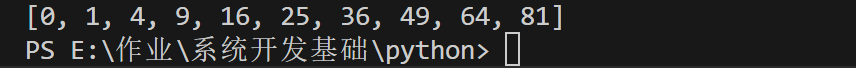
\includegraphics[width=\textwidth]{2112} % 确保文件名正确
    \caption{效果展示}
  
  \end{figure}
\end{itemize}
\end{enumerate}





%2.13LaTex=========================================================================%
\subsubsection{生成器表达式 }

\begin{enumerate}
  \item 创建一个生成器对象,该对象可以逐个生成0到9的平方数,而不需要将所有值存储在内存中
  \begin{itemize}
  \item 命令展示
  \begin{verbatim}

squares_generator = (x**2 for x in range(10))


for square in squares_generator:
    print(square)


    
  \end{verbatim}

  \item 效果展示
  \begin{figure}[H]
    \centering
    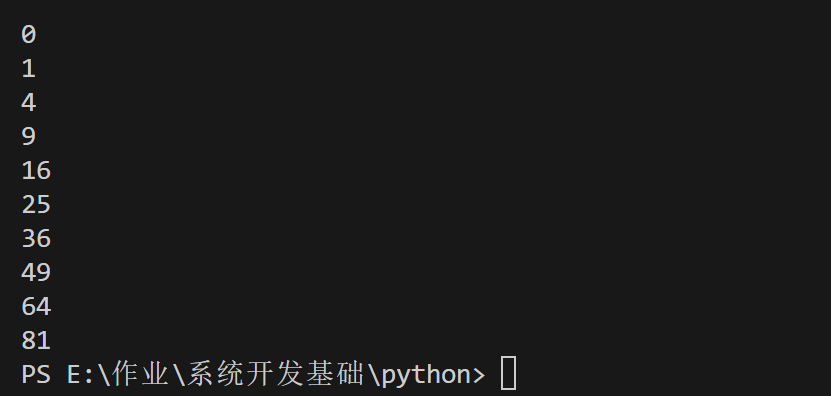
\includegraphics[width=\textwidth]{2113} % 确保文件名正确
    \caption{效果展示}
  
  \end{figure}
\end{itemize}
\end{enumerate}





%2.14LaTex=========================================================================%
\subsubsection{命名元组}

\begin{enumerate}
  \item 命名元组简单用法,提高可读性
  \begin{itemize}
  \item 命令展示
  \begin{verbatim}
 Point = namedtuple('Point', ['x', 'y'])
p = Point(1, 2)
print(p.x, p.y)

    
  \end{verbatim}

  \item 效果展示
  \begin{figure}[H]
    \centering
    
\includegraphics[width=\textwidth]{2114} % 确保文件名正确
    \caption{效果展示}
  
  \end{figure}
\end{itemize}
\end{enumerate}







%2.15LaTex=========================================================================%
\subsubsection{默认字典}

\begin{enumerate}
  \item 创建默认字典以避免KeyError
  \begin{itemize}
  \item 命令展示
  \begin{verbatim}
 from collections import defaultdict

default_dict = defaultdict(int)
default_dict['a'] += 1
print(default_dict)


    
  \end{verbatim}

  \item 效果展示
  \begin{figure}[H]
    \centering
    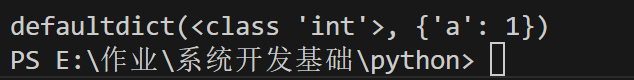
\includegraphics[width=\textwidth]{2115} % 确保文件名正确
    \caption{效果展示}
  
  \end{figure}
\end{itemize}
\end{enumerate}





































































%1.3LaTex=========================================================================%
  \subsection{Python视觉应用}
  {\color{blue}Python视觉应用展示}






%3.1LaTex=========================================================================%
\subsubsection{图像缩放}

\begin{enumerate}
  \item 使用PIL库对图像进行缩放,创建一个缩略图
  \begin{itemize}
  \item 命令展示
  \begin{verbatim}
from PIL import Image

def create_thumbnail(input_image_path, output_image_path, size=(128, 128)):
    with Image.open(input_image_path) as img:
        img.thumbnail(size)
        img.save(output_image_path)

create_thumbnail('path_to_large_image.jpg', 'path_to_thumbnail.jpg')

    
  \end{verbatim}

\item 效果展示
 
\begin{figure}[H]
    \centering
    \begin{subfigure}[b]{0.32\textwidth} % 将宽度设置为 0.32 以便三张图片可以并排
        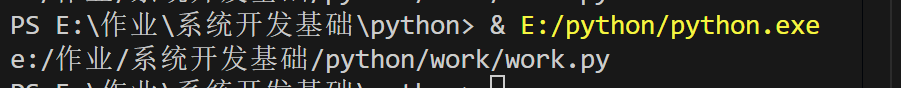
\includegraphics[width=\textwidth]{31} % 替换为您的第一张图片文件名
        \caption{1}
        \label{fig:left}
    \end{subfigure}
    \hfill
    \begin{subfigure}[b]{0.32\textwidth} % 将宽度设置为 0.32
        
\includegraphics[width=\textwidth]{32} % 替换为您的第二张图片文件名
        \caption{2}
        \label{fig:middle}
    \end{subfigure}
    \hfill
    \begin{subfigure}[b]{0.32\textwidth} % 将宽度设置为 0.32
        
\includegraphics[width=\textwidth]{33} % 替换为您的第三张图片文件名
        \caption{3}
        \label{fig:right}
    \end{subfigure}
    \caption{效果展示}
    \label{fig:three_images}
\end{figure}

  \end{itemize}
\end{enumerate}















%3.2LaTex=========================================================================%
\subsubsection{图像格式转换}

\begin{enumerate}
  \item 将一种图像格式转换为另一种格式,例如将JPEG转换为PNG。
  \begin{itemize}
  \item 命令展示
  \begin{verbatim}
  from PIL import Image

def convert_image_format(input_image_path, output_image_path, format='PNG'):
    with Image.open(input_image_path) as img:
        img.save(output_image_path, format=format)

convert_image_format('path_to_image.jpg', 'path_to_image.png')

    
  \end{verbatim}

\item 效果展示
 \begin{figure}[H]
    \centering
    \begin{subfigure}[b]{0.48\textwidth} % 将宽度设置为 0.48
        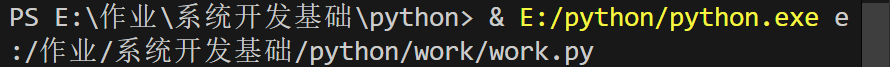
\includegraphics[width=\textwidth]{321} % 替换为您的第一张图片文件名
        \caption{1}
        \label{fig:left}
    \end{subfigure}
    \hfill
    \begin{subfigure}[b]{0.48\textwidth} % 将宽度设置为 0.48
        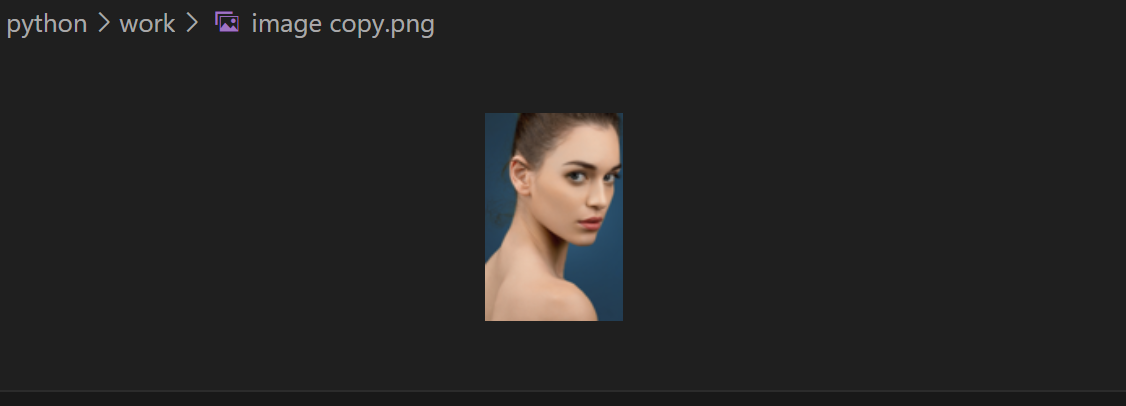
\includegraphics[width=\textwidth]{322} % 替换为您的第二张图片文件名
        \caption{2}
        \label{fig:right}
    \end{subfigure}
    \caption{效果展示}
    \label{fig:two_images}
\end{figure}

  \end{itemize}
\end{enumerate}




















%3.3LaTex=========================================================================%
\subsubsection{图像旋转}

\begin{enumerate}
  \item 使用PIL库对图像进行90度旋转
  \begin{itemize}
  \item 命令展示
  \begin{verbatim}
from PIL import Image

def rotate_image(input_image_path, output_image_path):
    with Image.open(input_image_path) as img:
        rotated_img = img.rotate(90)
        rotated_img.save(output_image_path)

rotate_image('path_to_image.jpg', 'path_to_rotated_image.jpg')

    
  \end{verbatim}
\item 效果展示
  \begin{figure}[H]
    \centering
    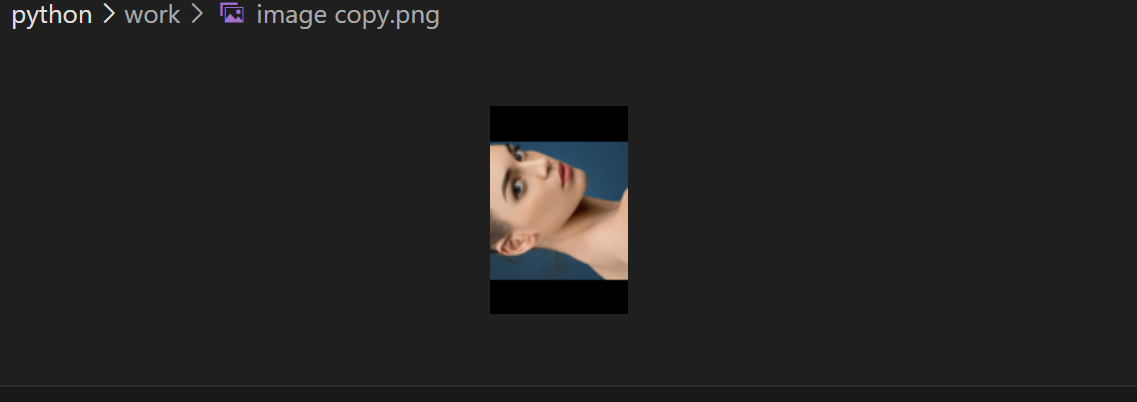
\includegraphics[width=\textwidth]{333} % 替换为您的图片文件名
    \caption{效果展示}
  \end{figure}
  \end{itemize}
\end{enumerate}
























%3.4LaTex=========================================================================%
\subsubsection{图像灰度化}

\begin{enumerate}
  \item 将彩色图像转换为灰度图像
  \begin{itemize}
  \item 命令展示
  \begin{verbatim}
from PIL import Image

def convert_to_grayscale(input_image_path, output_image_path):
    with Image.open(input_image_path) as img:
        grayscale_img = img.convert('L')
        grayscale_img.save(output_image_path)

convert_to_grayscale('path_to_color_image.jpg', 'path_to_grayscale_image.jpg')

    
  \end{verbatim}

 
\item 效果展示
  \begin{figure}[H]
    \centering
    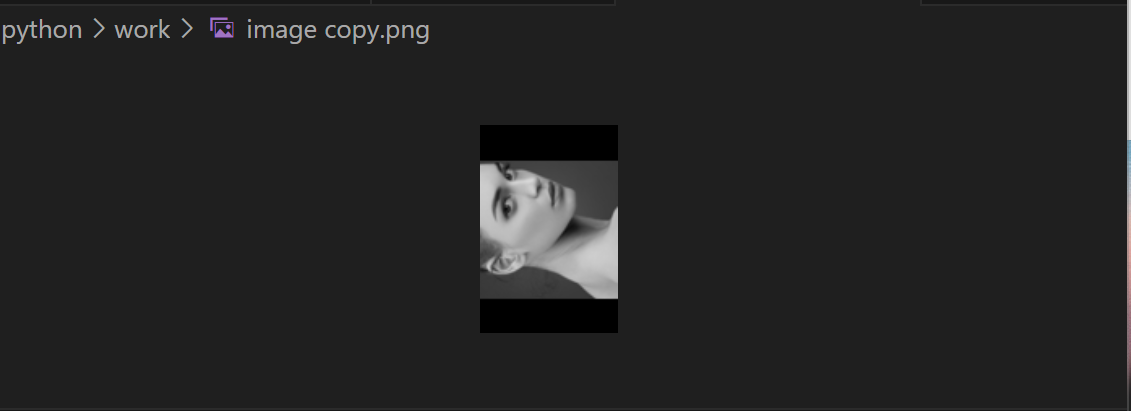
\includegraphics[width=\textwidth]{334} % 替换为您的图片文件名
    \caption{效果展示}
  \end{figure}
  \end{itemize}
\end{enumerate}

















%3.5LaTex=========================================================================%
\subsubsection{图像直方图均衡化}

\begin{enumerate}
  \item 使用NumPy和PIL库对图像进行直方图均衡化,以改善图像的对比度。
  \begin{itemize}
  \item 命令展示
  \begin{verbatim}
import numpy as np
from PIL import Image
import matplotlib.pyplot as plt

def histogram_equalization(image):
    # 将图像转换为灰度图像
    gray_image = image.convert('L')
    img_array = np.array(gray_image)

    # 计算直方图
    hist, bins = np.histogram(img_array.flatten(), bins=256, range=[0,256])

    # 计算累积直方图
    cdf = hist.cumsum()
    cdf_normalized = cdf * hist.max() / cdf.max()  # 归一化

    # 使用线性插值进行直方图均衡化
    cdf_m = np.ma.masked_equal(cdf, 0)  # 避免除以零
    cdf_m = (cdf_m - cdf_m.min()) * 255 / (cdf_m.max() - cdf_m.min())  # 归一化
    cdf = np.ma.filled(cdf_m, 0).astype('uint8')  # 填充掩码

    # 应用直方图均衡化
    img_equalized = cdf[img_array]
    
    return Image.fromarray(img_equalized)

# 打开图像
image_path = 'E:\作业\系统开发基础\python\work\image.png'  # 替换为你的图像路径
image = Image.open(image_path)

# 进行直方图均衡化
equalized_image = histogram_equalization(image)

# 显示原图和均衡化后的图像
plt.figure(figsize=(12, 6))
plt.subplot(1, 2, 1)
plt.title('Original Image')
plt.imshow(image)
plt.axis('off')

plt.subplot(1, 2, 2)
plt.title('Histogram Equalized Image')
plt.imshow(equalized_image, cmap='gray')
plt.axis('off')

plt.show()


    
  \end{verbatim}


\item 效果展示
  \begin{figure}[H]
    \centering
    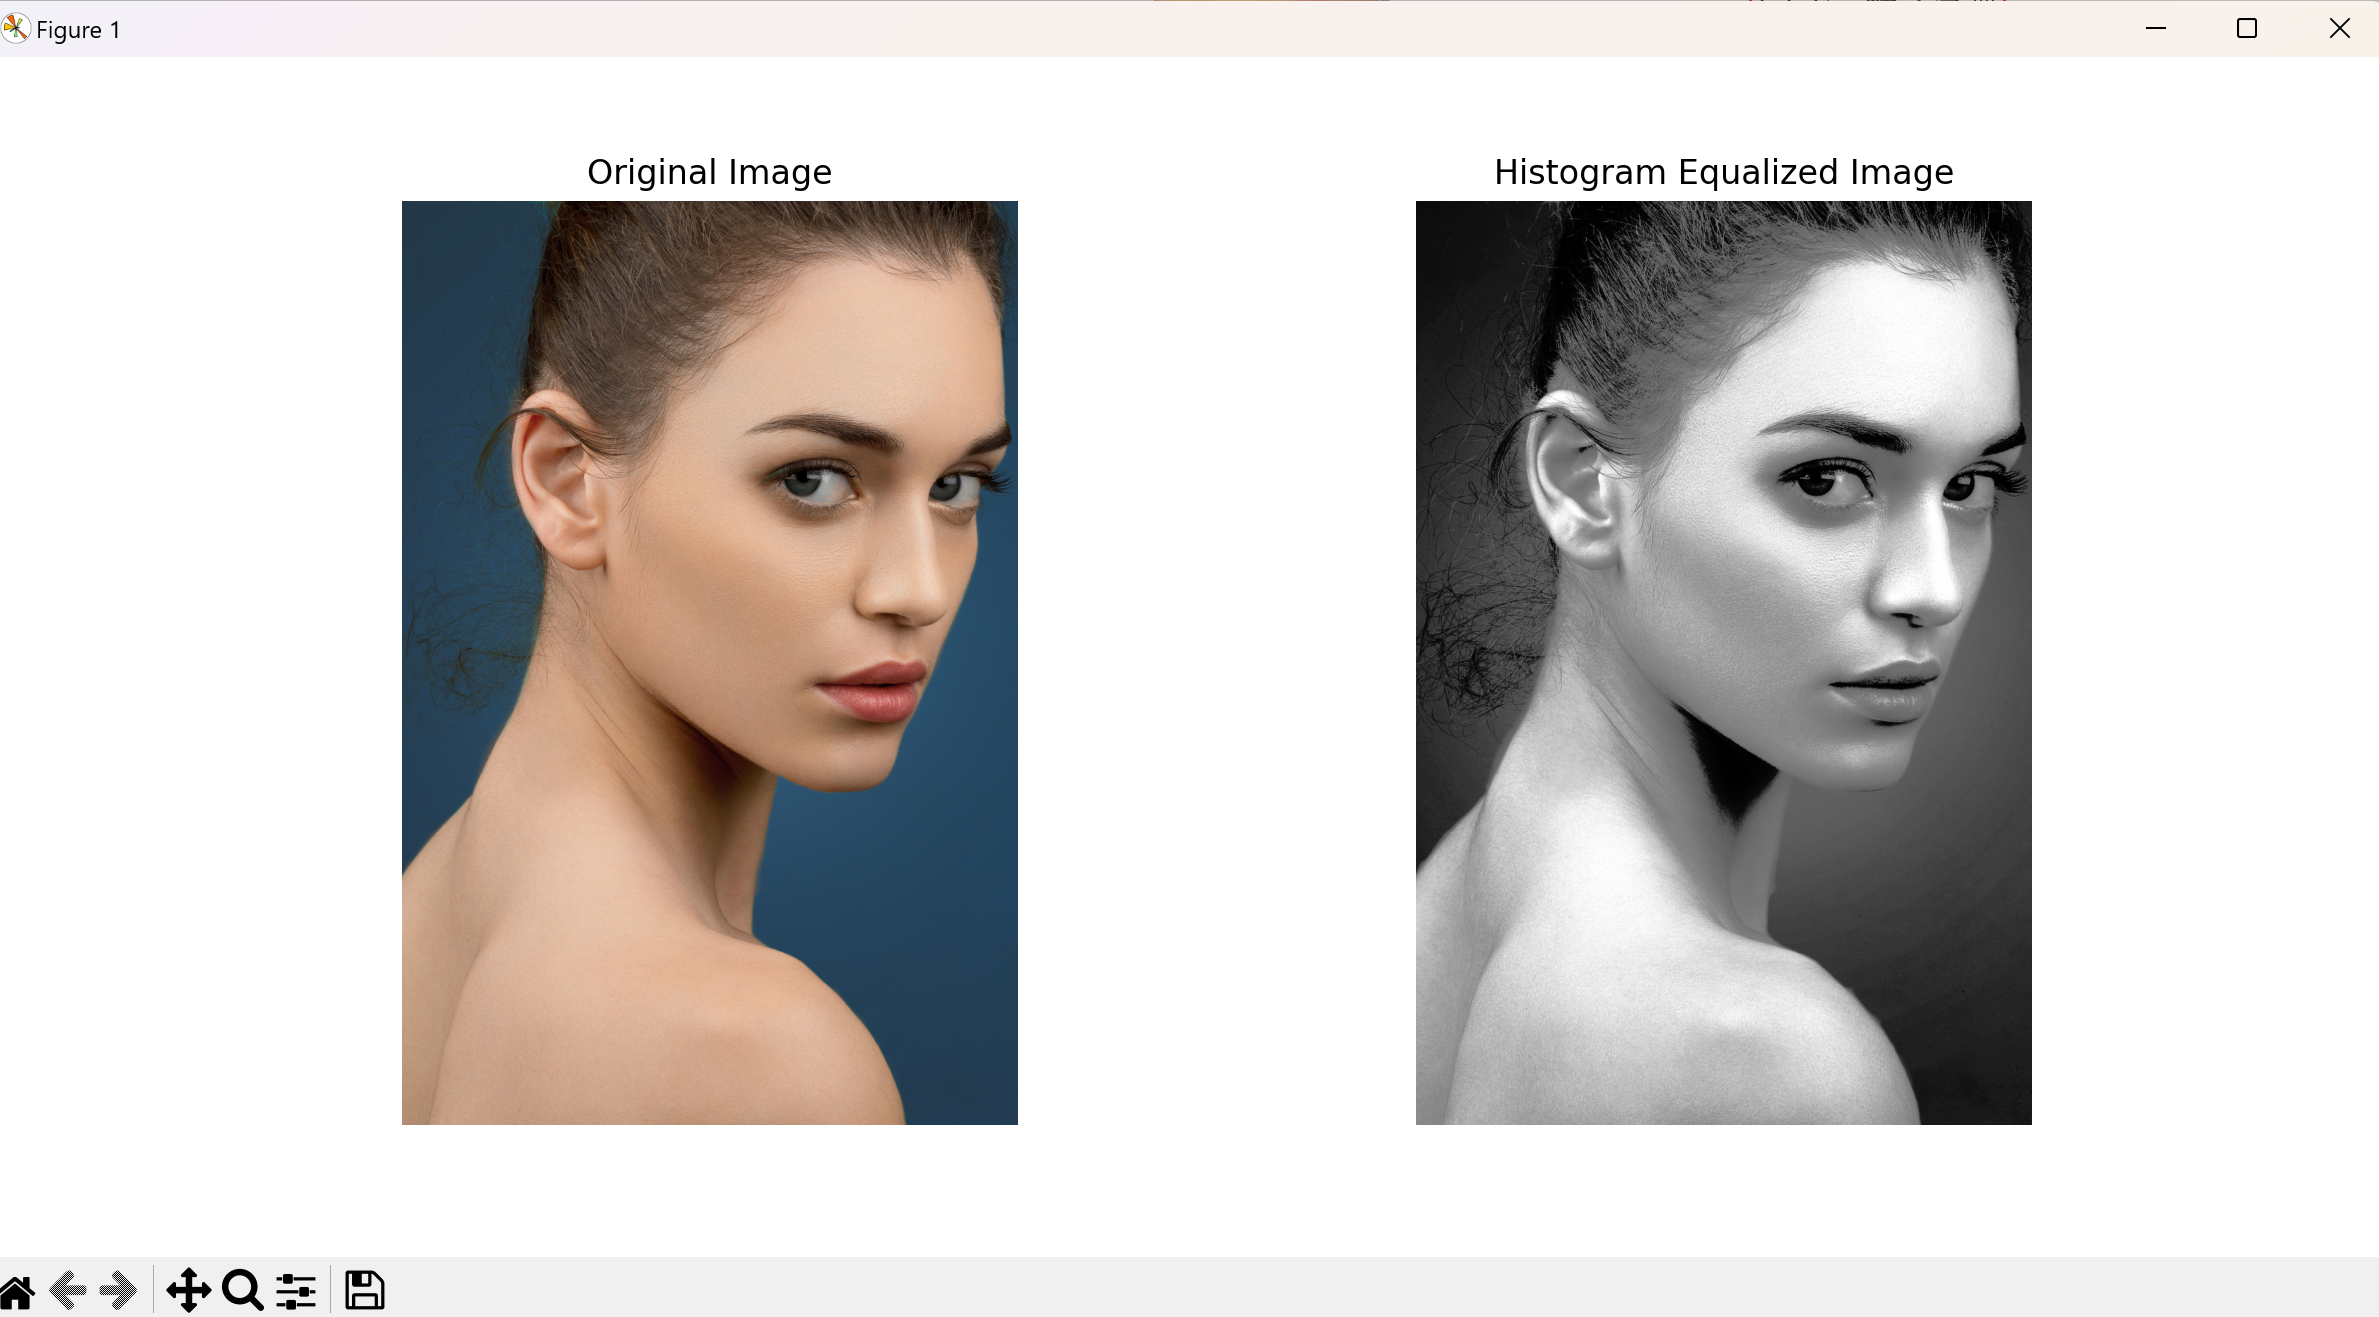
\includegraphics[width=\textwidth]{335} % 替换为您的图片文件名
    \caption{效果展示}
  \end{figure}
  \end{itemize}
\end{enumerate}





















%3.6LaTex=========================================================================%























%3.7LaTex=========================================================================%




















%3.8LaTex=========================================================================%





















%3.9LaTex=========================================================================%




















%3.10LaTex=========================================================================%






























%1.2.16表格==================================================%
 \section{困难与解决方案} \subsection{命令行环境}

\begin{enumerate} \item \begin{itemize} \item 问题:系统无法识别 tumx 命令 \item 解决方案:可以使用 apt 来安装 tmux \end{itemize}\item \begin{itemize} \item 问题:在不同操作系统上使用命令行工具时,命令和选项不一致,导致混淆。 \item 解决方案:查看跨平台的命令行使用指南 \end{itemize} \item \begin{itemize} \item 问题:命令行工具的性能问题,执行大文件时速度缓慢。 \item 解决方案:优化命令参数设置,使用更高效的算法,或使用并行处理工具(如 GNU Parallel)来提升性能。 \end{itemize} \item \begin{itemize} \item 问题:ssh失败 \item 解决方案:安装 OpenSSH 服务器。 \end{itemize}  \end{enumerate}

\subsection{Python入门基础} \begin{enumerate} \item \begin{itemize} \item 问题:空格没有把握好,老是报错 \item 解决方案:多加练习 \end{itemize} \end{enumerate}

\subsection{Python视觉应用}

\begin{enumerate} \item \begin{itemize} \item 问题:在图像处理项目中,缺乏对图像格式和编码的了解。 \item 解决方案:通过网上学习了解不同图像格式的对比及其优缺点 \end{itemize} \item \begin{itemize} \item 问题:缺乏使用深度学习进行图像识别的基础知识。 \item 解决方案:学习基本知识(如 TensorFlow 和 PyTorch)的入门教程,结合实际应用案例,逐步理解深度学习的基本原理和应用。 \end{itemize} \item \begin{itemize} \item 问题:不会下载图像处理所需要的各种库 \item 解决方案:在网上学习方法来解决 \end{itemize} \end{enumerate}

%1.2.16表格==================================================% 
\section{心得体会} \begin{itemize} \item 通过解决命令行环境的问题,我对系统配置有了更深入的理解,并提升了自己排错的能力。 \item 在学习 Python 基础知识的过程中,我认识到代码的清晰性和注释的重要性,这让我在编写代码时更加注重可读性。同时我对字典。列表等有了更深入的认识 \item 参与 Python 视觉应用的项目让我对图像处理有了初步的认识,激发了我进一步探索这一领域的兴趣。\end{itemize}



  %1.2.16表格==================================================%

  \section{github网址}
\href{https://github.com/KeepingMoving/work1.git}{GitHub仓库}
https://github.com/KeepingMoving/work1.git
 










\end{document}
